

\chapter{Material and methods}

%  Everything that is mentioned in results, has to be mentioned here
%  Everybody who reads thesis, must be able to reproduce the experiment/study
% o Describe all materials, devices and methods, which were used in your work
% o if you describe a device, start with the brand name followed by the company name, city and country in parentheses: e.g. "... a VersaHD (Elekta AB, Stockholm, Sweden) was used in ...".
% o Provide some information on each device
%  e.g Linac, which energies were used, what was the field size, what was the leaf width, how is the linac calibrated, ...;
%  e.g. Detector array: which type of detector, how many detectors, what is the resolution, energy dependence, linearity,...;
%  e.g. Panning systems: software version, algorithms, settings used in this study
%  e.g. software: version, functionality
% o Also describe used data (patient cohort) even if they were taken from other studies

\section{Scanners}

The radiation oncology department of the Vienna General Hospital (AKH) owns a open-bore, c-arm MRI scanner and a CT scanner (used as reference).
They are listed in Table \ref{tab:scanners}.

\begin{table}[h]
\centering
\begin{tabular}{llll}
System	& product name	& company	& coil [internal W x H]		\\
\toprule
MRI	& Magnetom C!	& Siemens	& Body/Spine Array Coil XL	\\
	&		&		& [50 x 30.5 cm (19.7 x 12 in)]	\\
CT	&		&		& --------
\end{tabular}
\caption{used scanners}
\label{tab:scanners}
\end{table}

\subsection{MRI scanner - field distribution}
\label{sec:magnetom}

The Magnetom C! MRI scanner comes with a handbook which contains diagrams of the magnetic field strength (fig. \ref{fig:strength_side}), and its gradient (fig. \ref{fig:gradient_side}, \ref{fig:gradient_top}, and  \ref{fig:gradient_front}).
Figure \ref{fig:scanner} shows an image and different views of the scanner and the planes along which the field strength and gradient are displayed.

\begin{figure}[!htb]
\centering
  \begin{subfigure}[b]{0.4\textwidth}
	\centering
	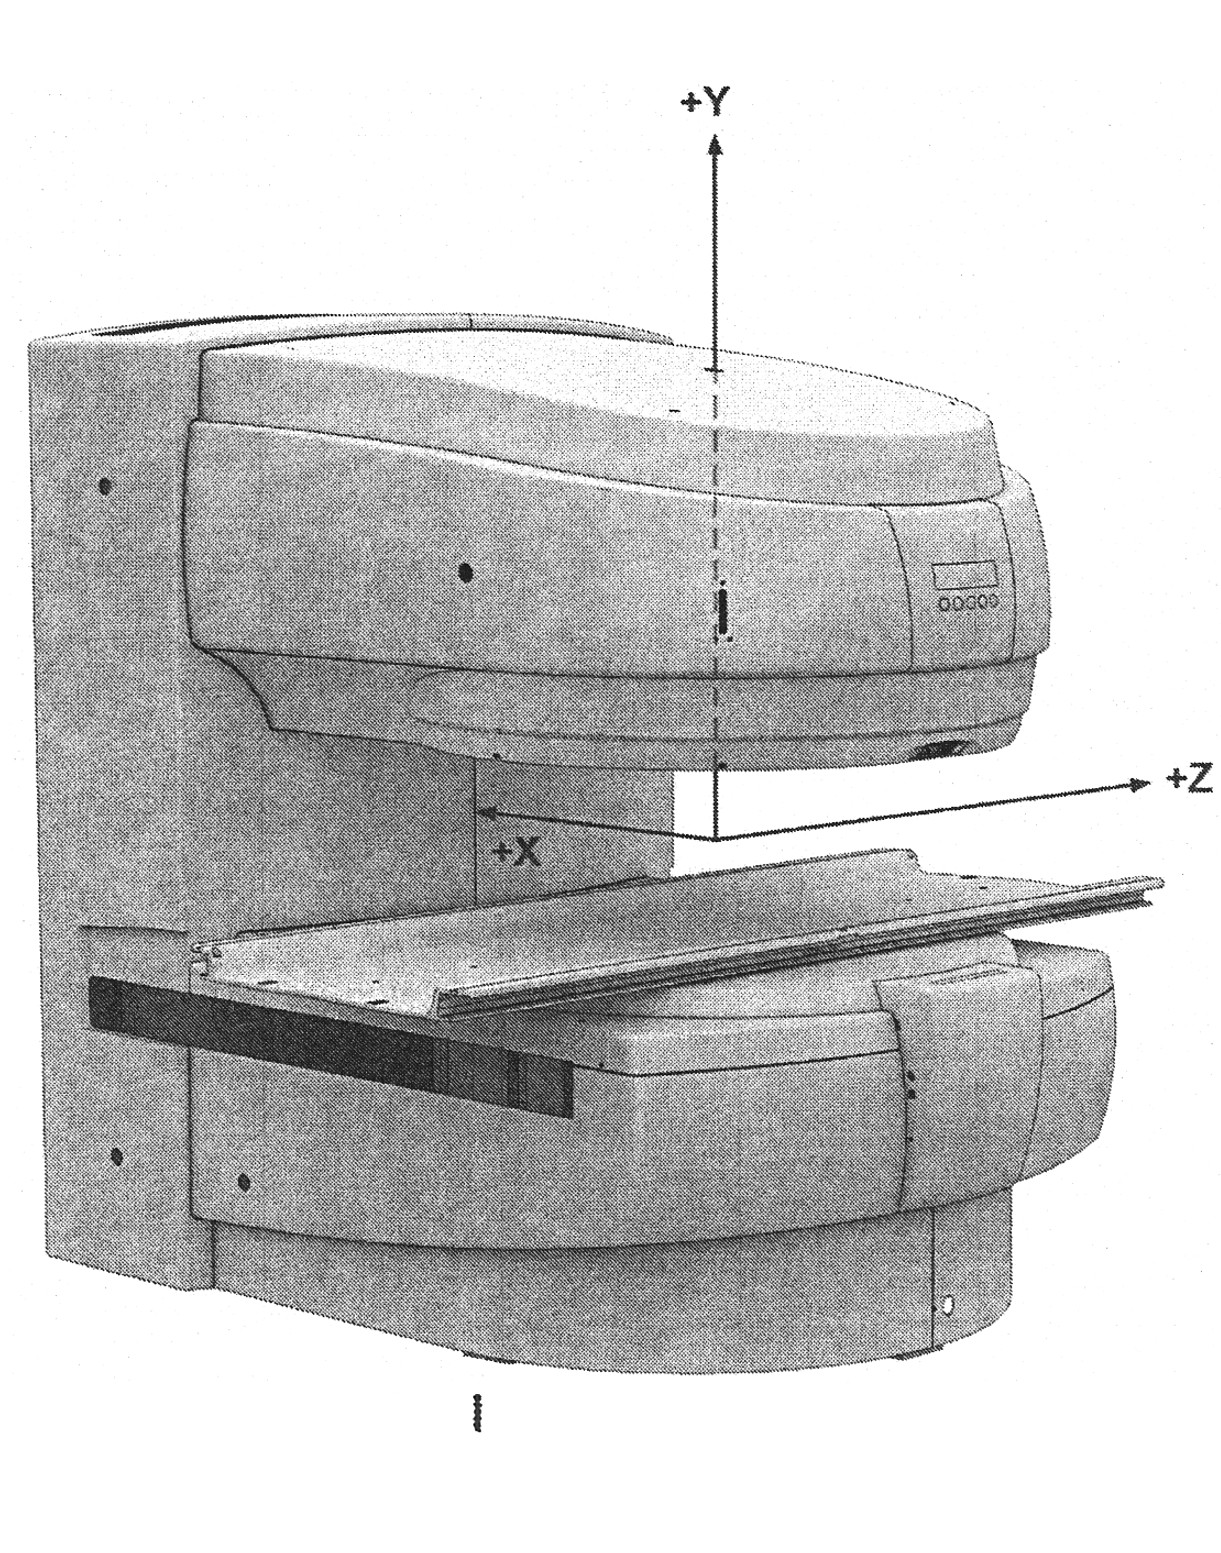
\includegraphics[scale=0.7]{scanner/scanner_img.jpg}
	\caption{Image of scanner\\ x,y, \& z -axis}
	\label{fig:scanner_image}
  \end{subfigure}
    \hfill
  \begin{subfigure}[b]{0.4\textwidth}
  	\centering
    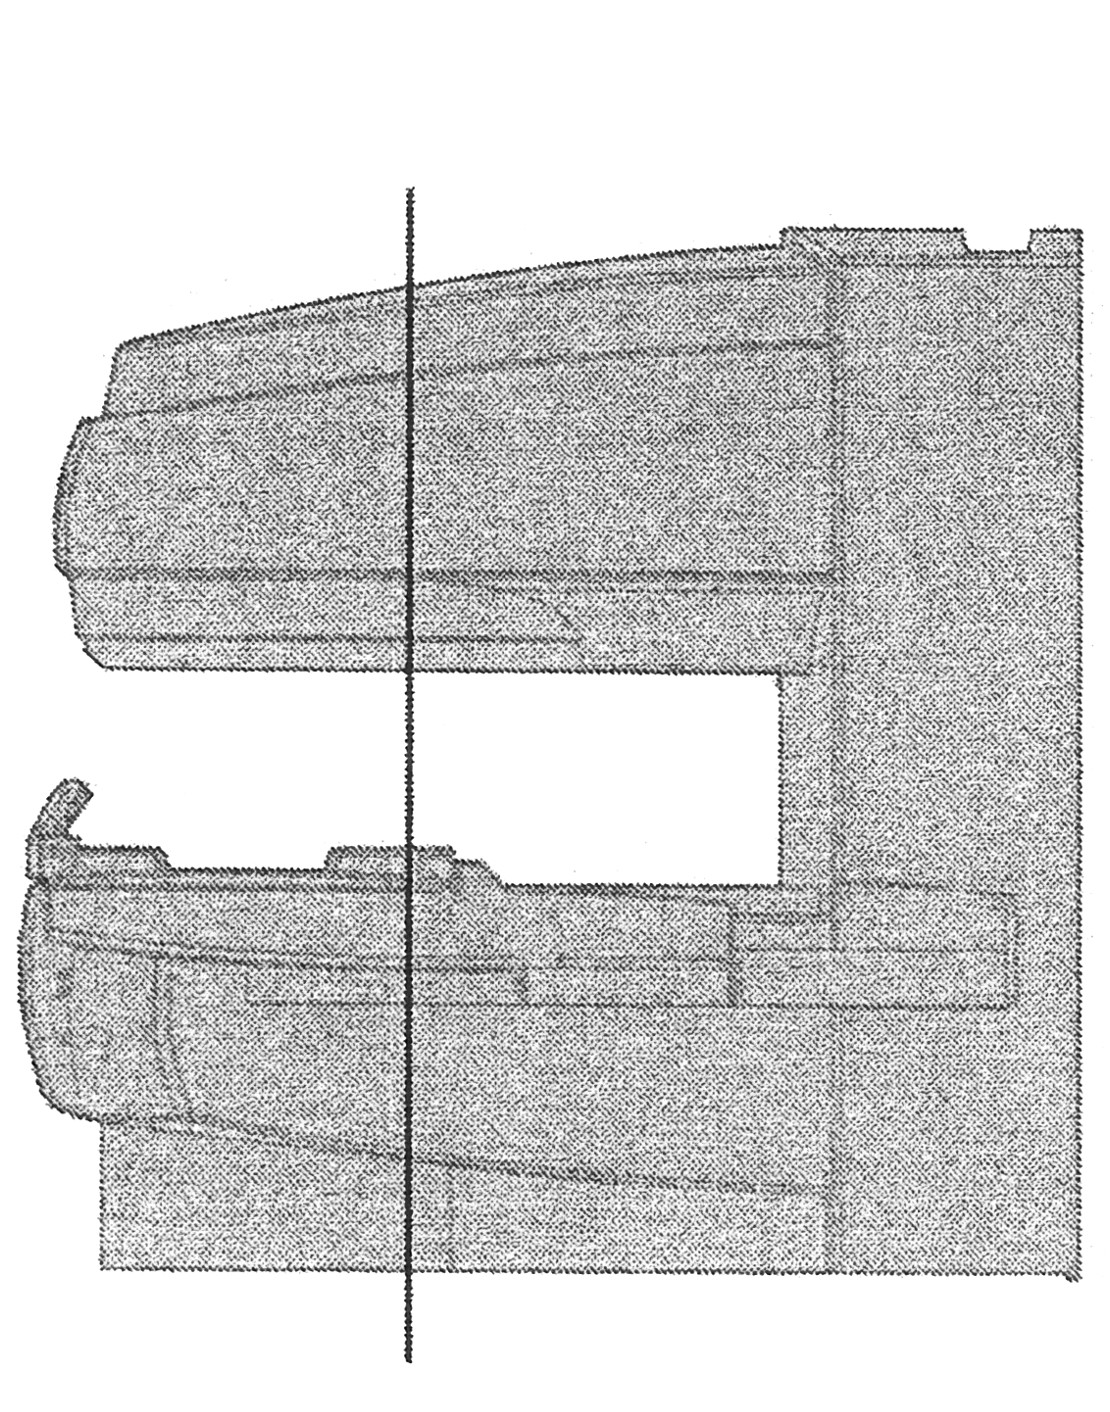
\includegraphics[scale=0.7]{scanner/scanner_front.jpg}
    \caption{side view along z-axis,\\ black line represents plane for front view (see fig. \ref{fig:gradient_front})}
    \label{fig:scanner_front}
  \end{subfigure}
  
  \begin{subfigure}[b]{0.4\textwidth}
   	\centering
   	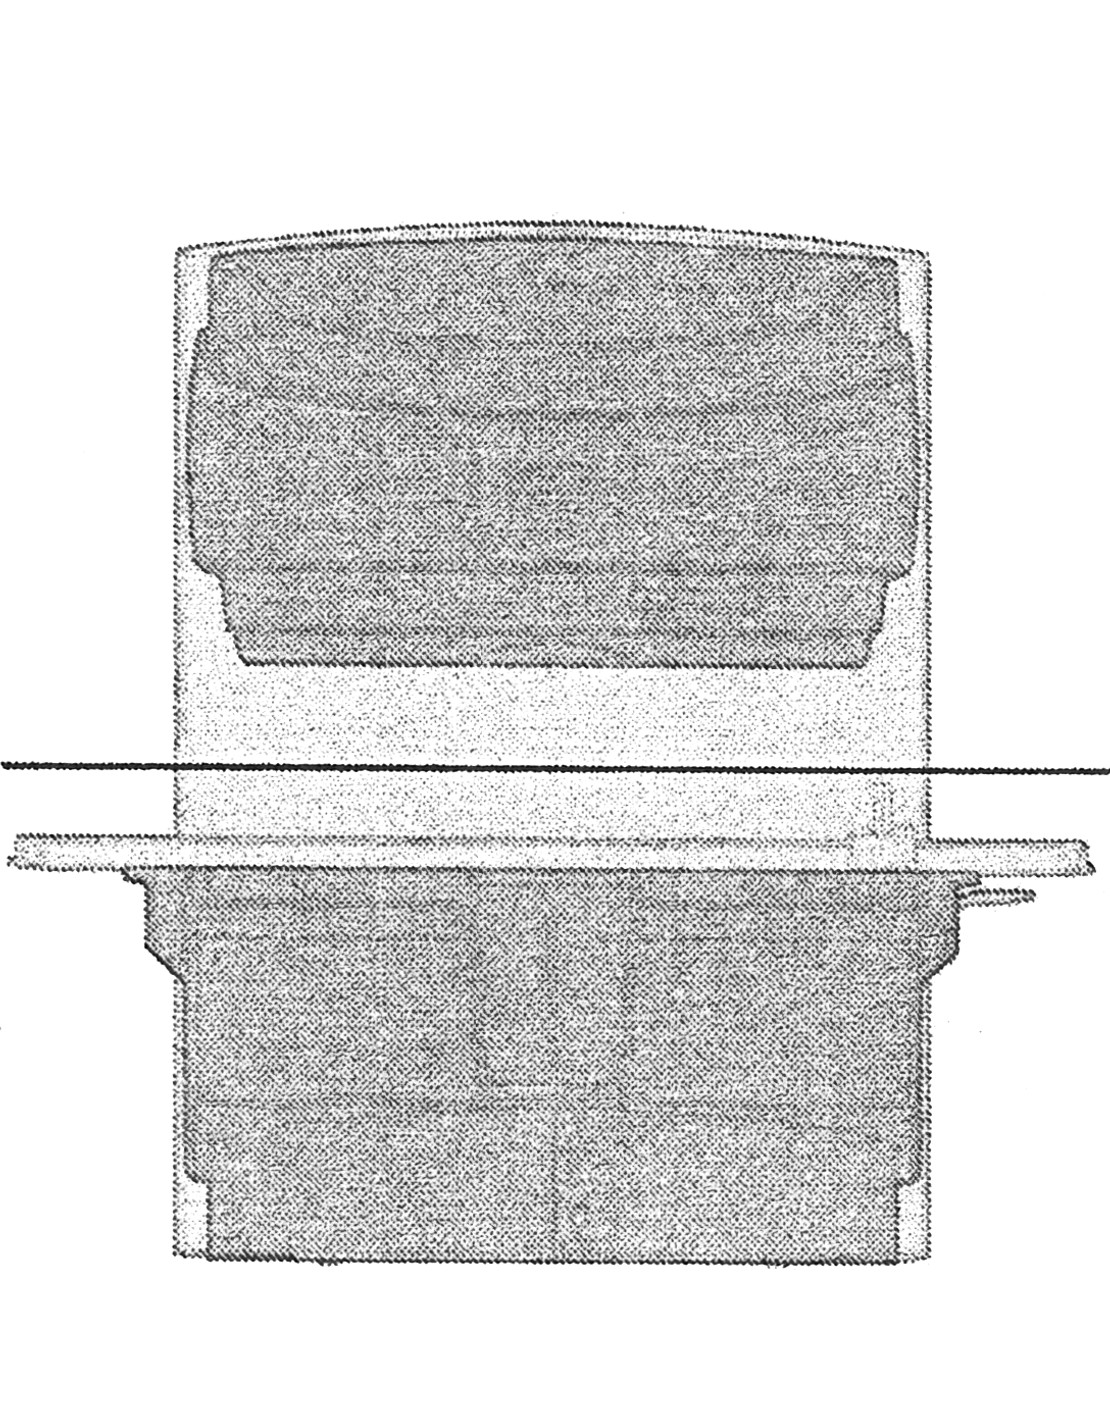
\includegraphics[scale=0.7]{scanner/scanner_top.jpg}
   	\caption{front view along x-axis,\\ black line represents plane for top view (see fig. \ref{fig:gradient_top})}
   	\label{fig:scanner_top}
  \end{subfigure}
    \hfill
  \begin{subfigure}[b]{0.4\textwidth}
  	\centering
  	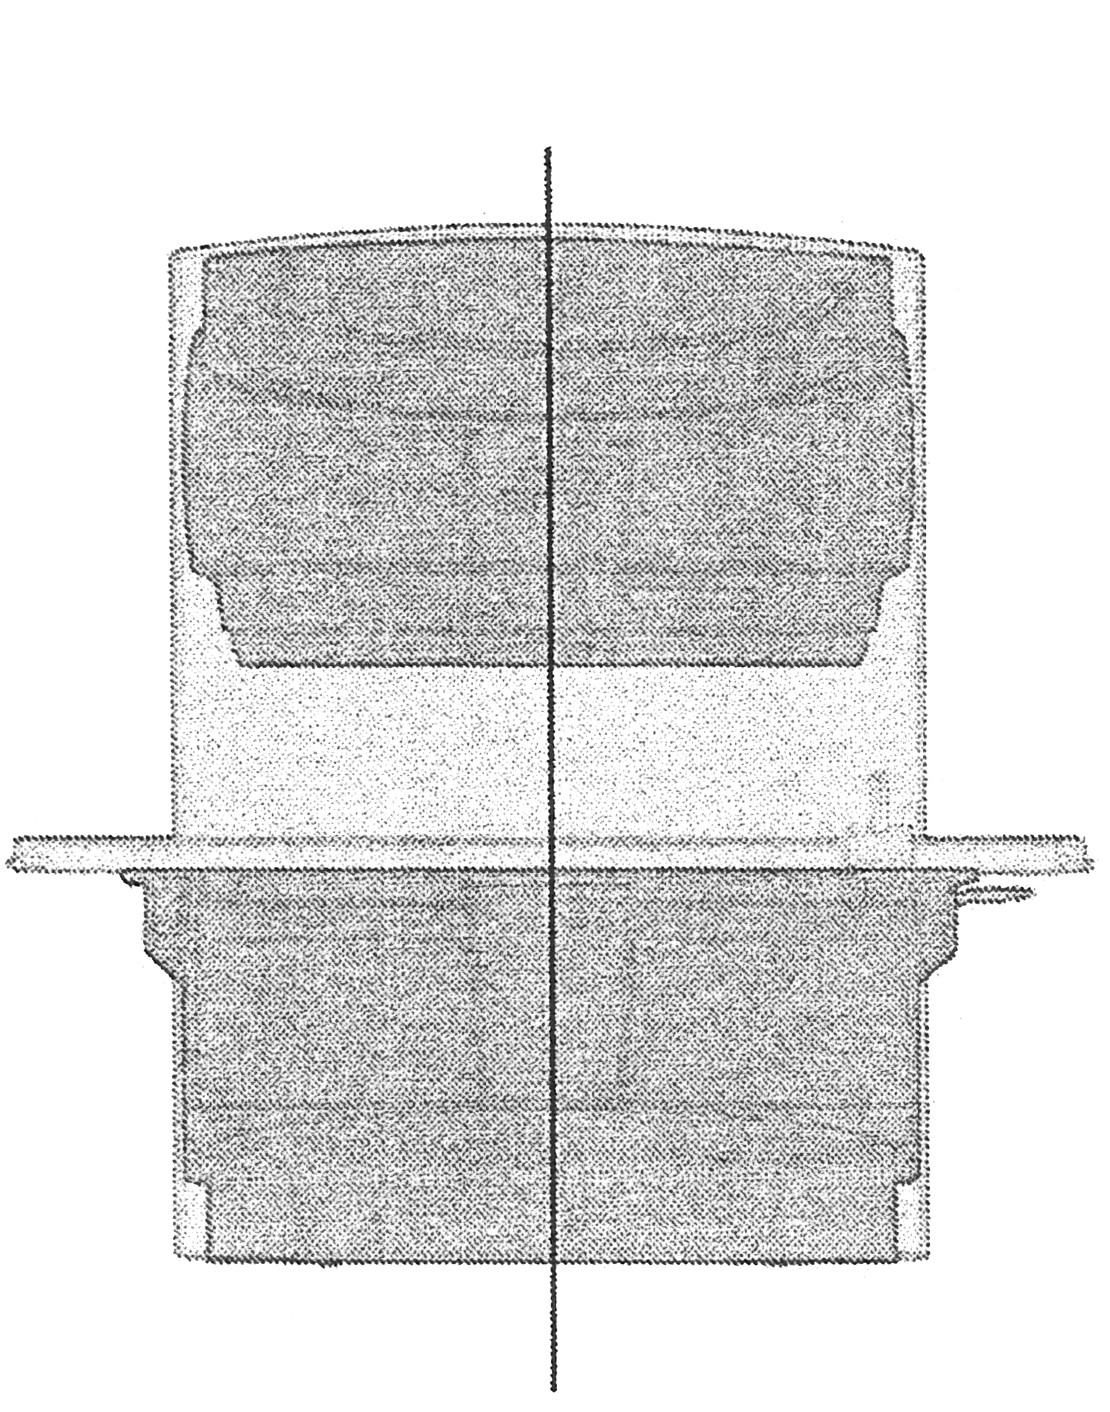
\includegraphics[scale=0.7]{scanner/scanner_side.jpg}
  	\caption{front view along x-axis,\\ black line represents plane for side view (see fig. \ref{fig:gradient_side} and \ref{fig:strength_side})}
  	\label{fig:scanner_side}
  \end{subfigure}
  \caption{Magnetom C! \cite{magnetom_handbook}}
  \label{fig:scanner}
\end{figure}

%diagrams as individual figures:
\begin{figure}[!htb]
  	\centering
      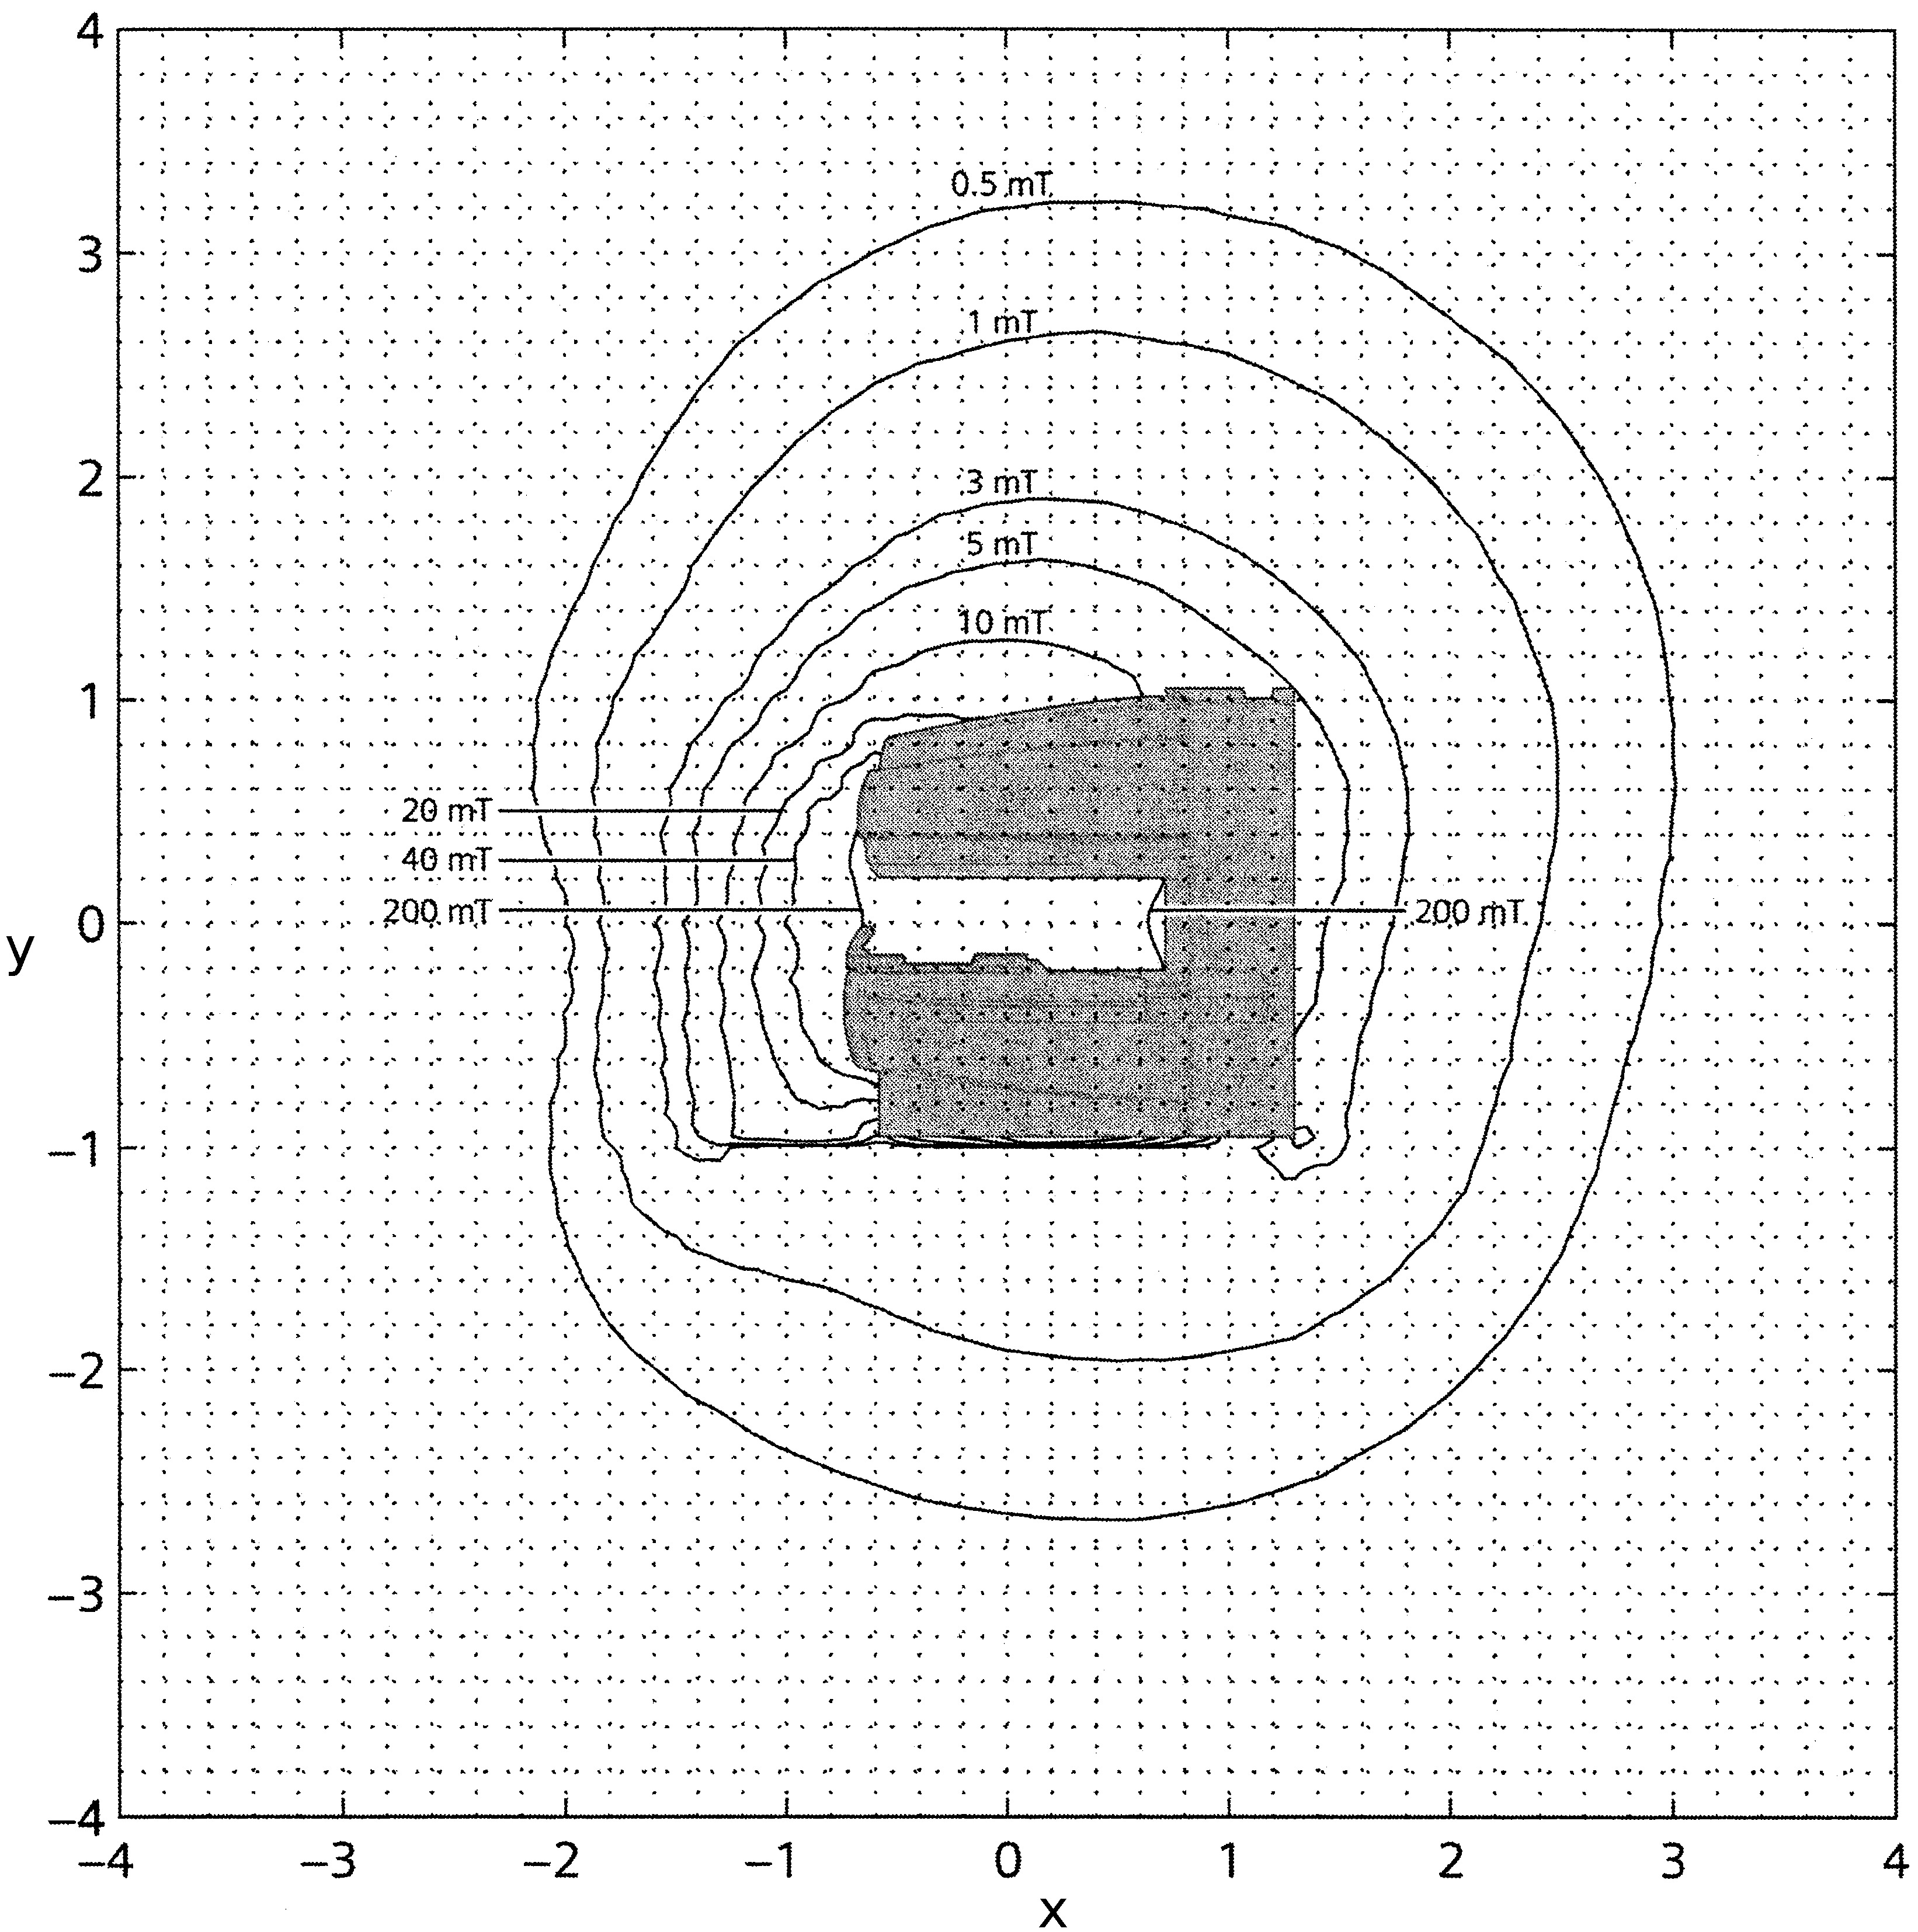
\includegraphics[scale=1.1]{scanner/scanner_field-strength.jpg}
      \caption{Magnetom C! field strength\\ side view along z-axis (see fig. \ref{fig:scanner_side}) \cite{magnetom_handbook}}
    \label{fig:strength_side}
\end{figure}

\begin{figure}[!htb]
    	\centering
        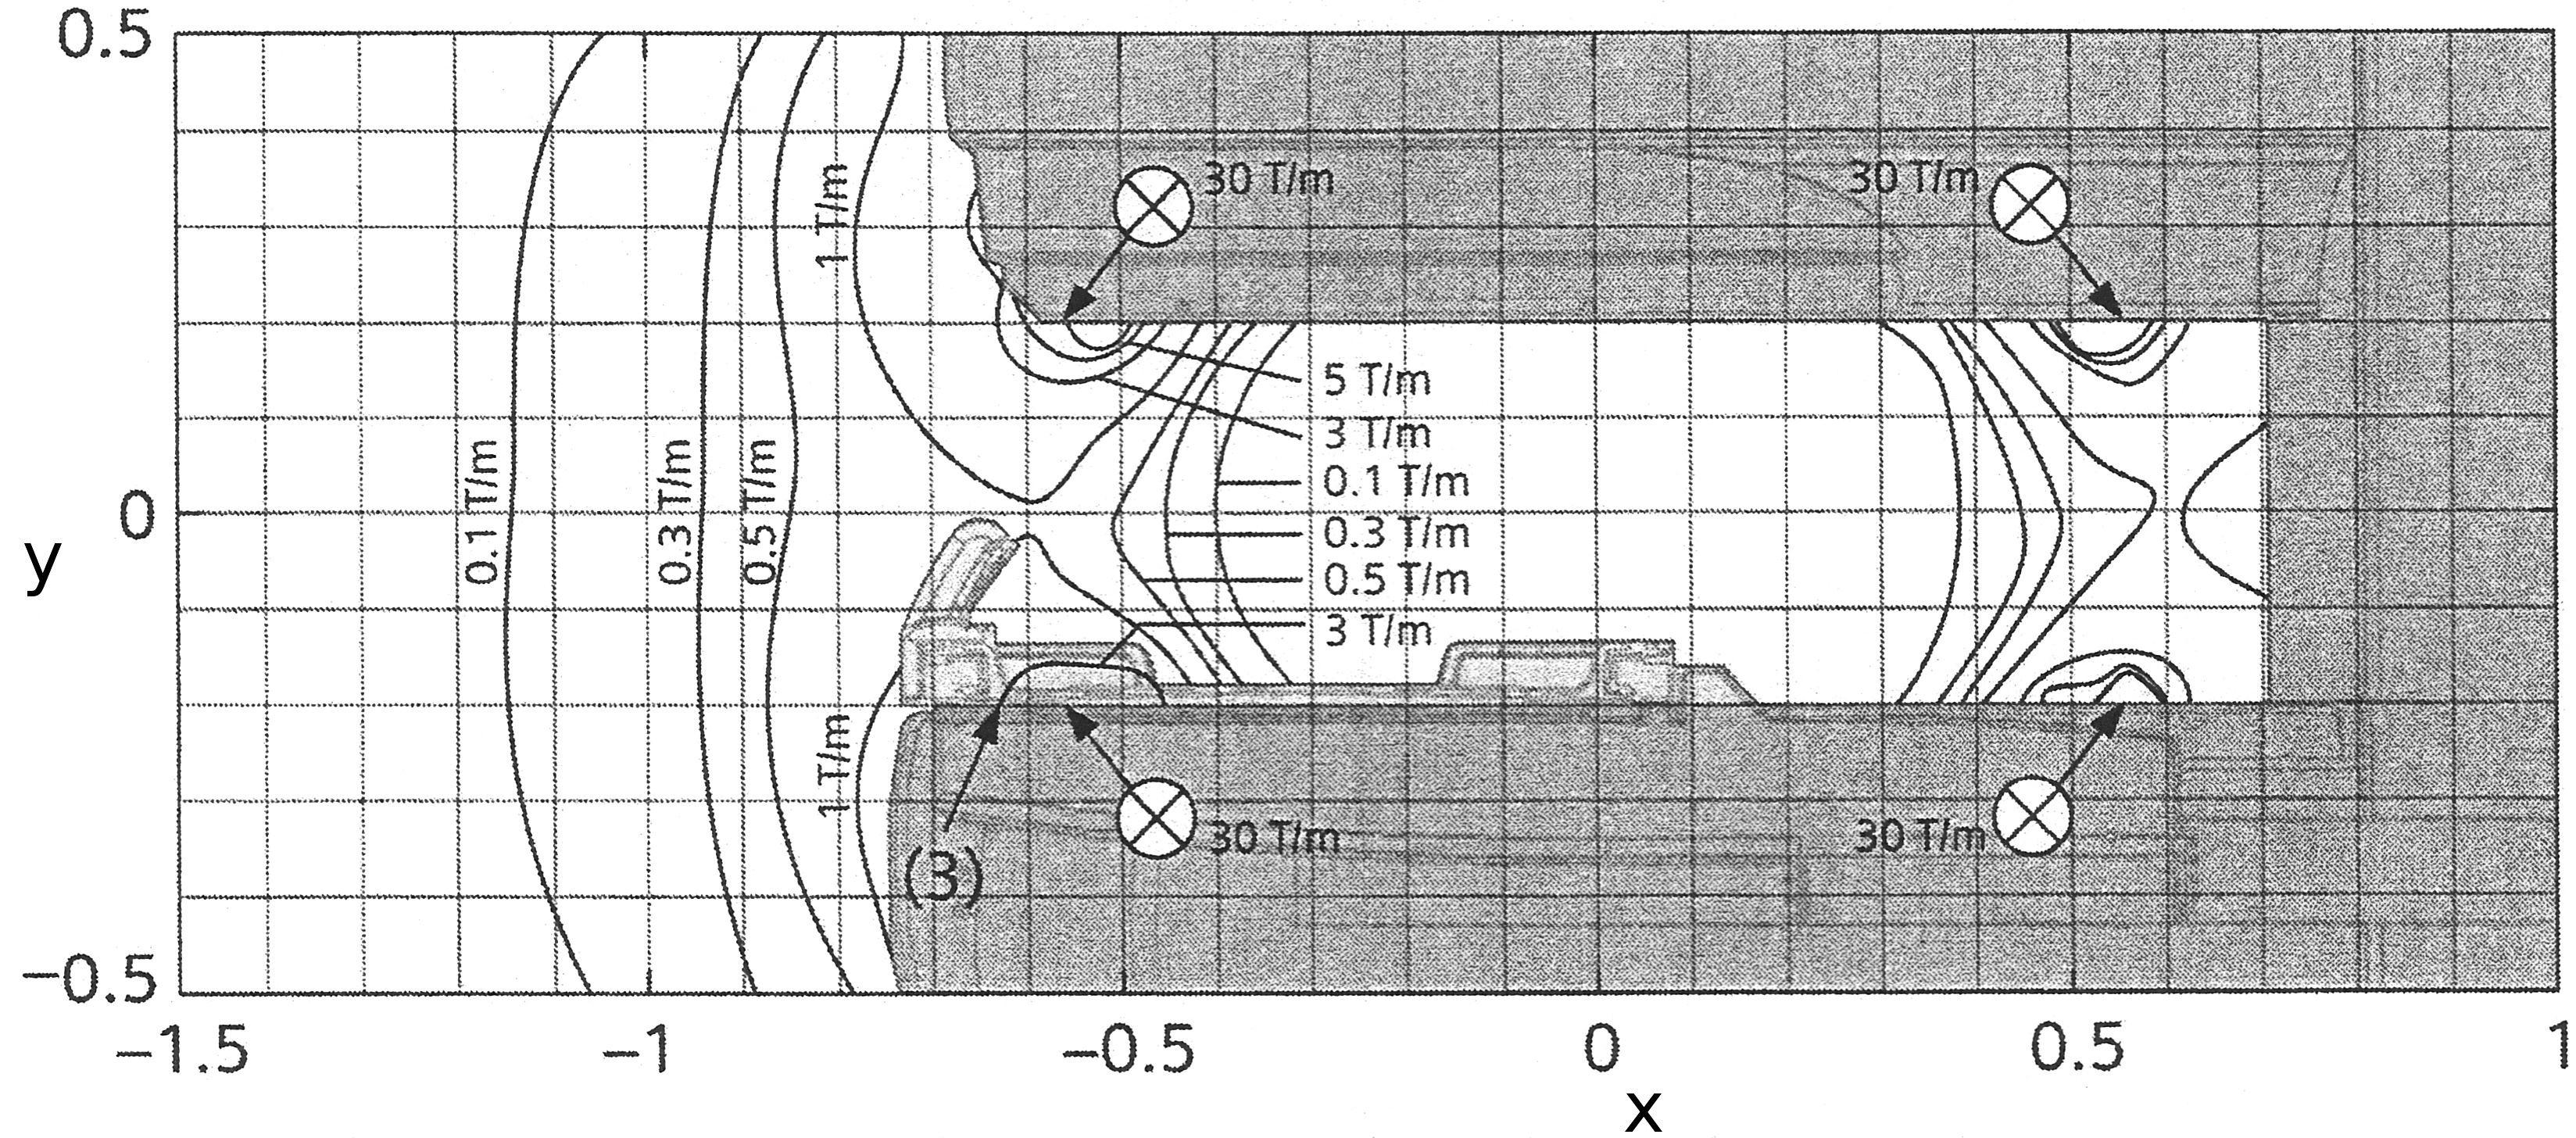
\includegraphics[scale=1.1]{scanner/scanner_gradient-side.jpg}
        \caption{Magnetom C! field gradient\\ side view along z-axis (see fig. \ref{fig:scanner_side}) \cite{magnetom_handbook}}
        \label{fig:gradient_side}
\end{figure}

\begin{figure}[!htb]
  	\centering
    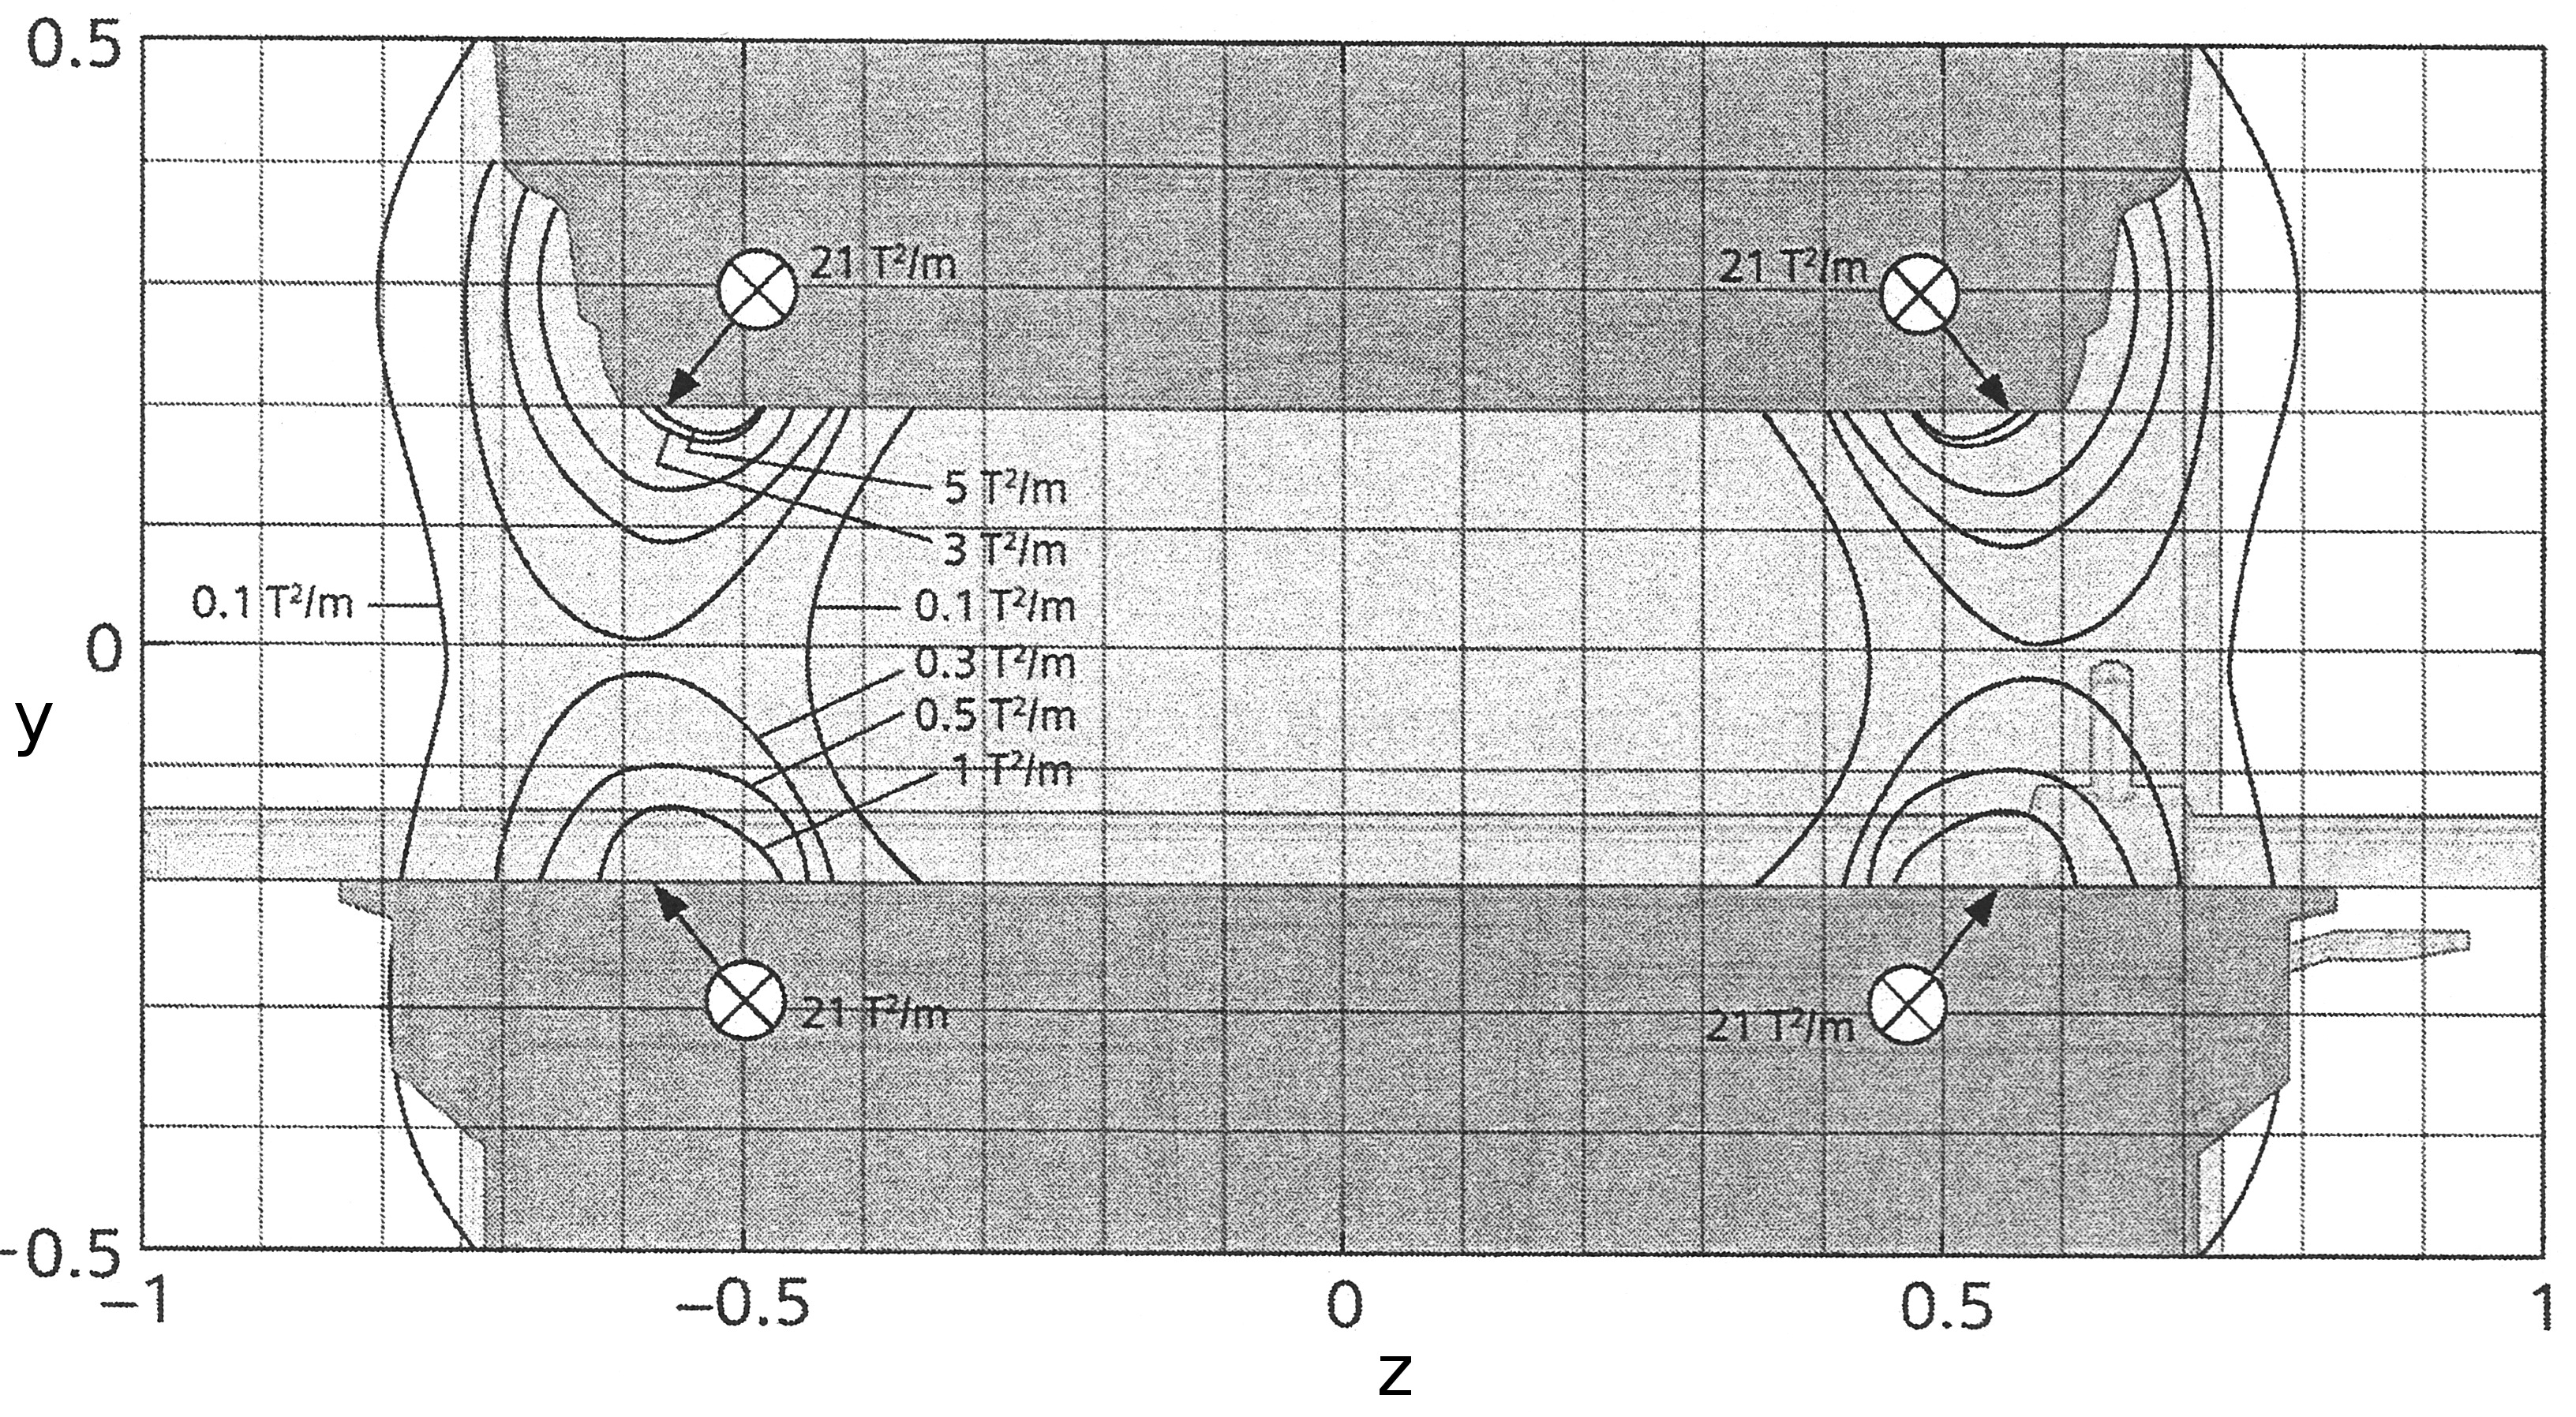
\includegraphics[scale=1.1]{scanner/scanner_gradient-front.jpg}
    \caption{Magnetom C! field gradient\\ front view along x-axis (see fig. \ref{fig:scanner_front}) \cite{magnetom_handbook}}
    \label{fig:gradient_front}
    \end{figure}

\begin{figure}[!htb]
  	\centering
    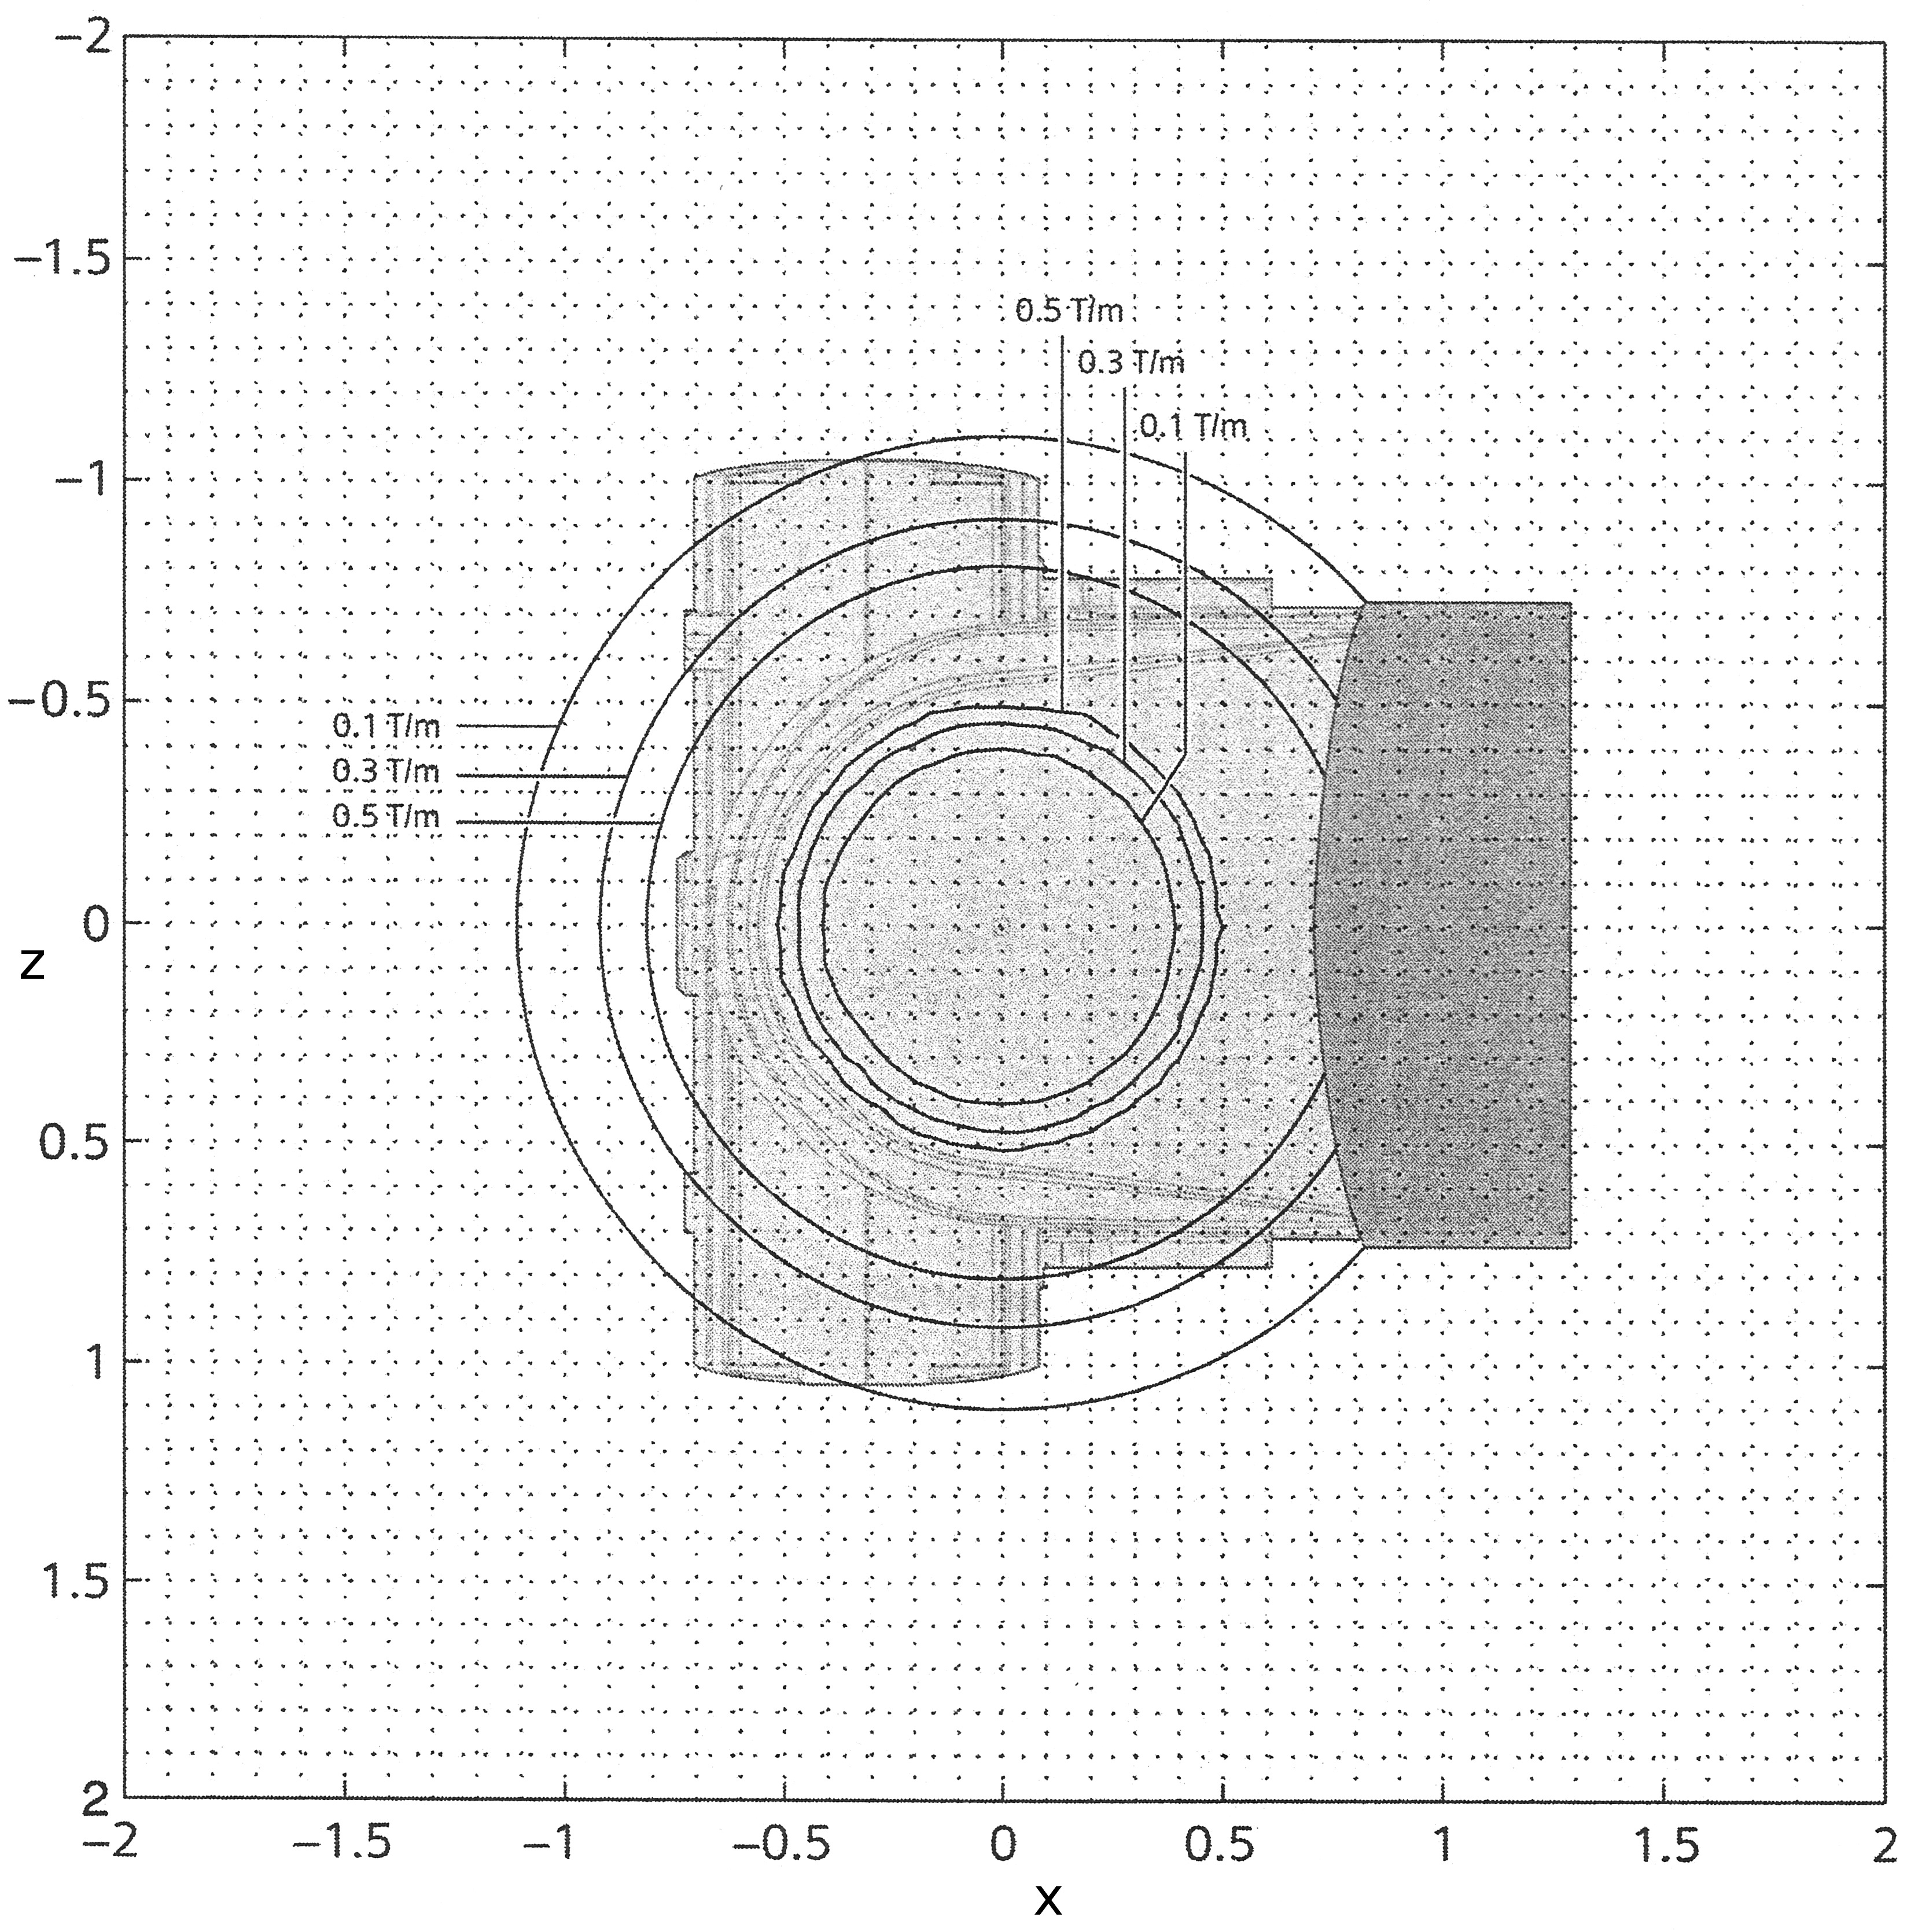
\includegraphics[scale=1.1]{scanner/scanner_gradient-top.jpg}
    \caption{Magnetom C! field gradient\\ top view along y-axis (see fig. \ref{fig:scanner_top}) \cite{magnetom_handbook}}
    \label{fig:gradient_top}
\end{figure}


% diagrams as sets of subfigures:
%\begin{figure}[!htb]
%\centering
%  \begin{subfigure}[b]{\textwidth}
%  	\centering
%    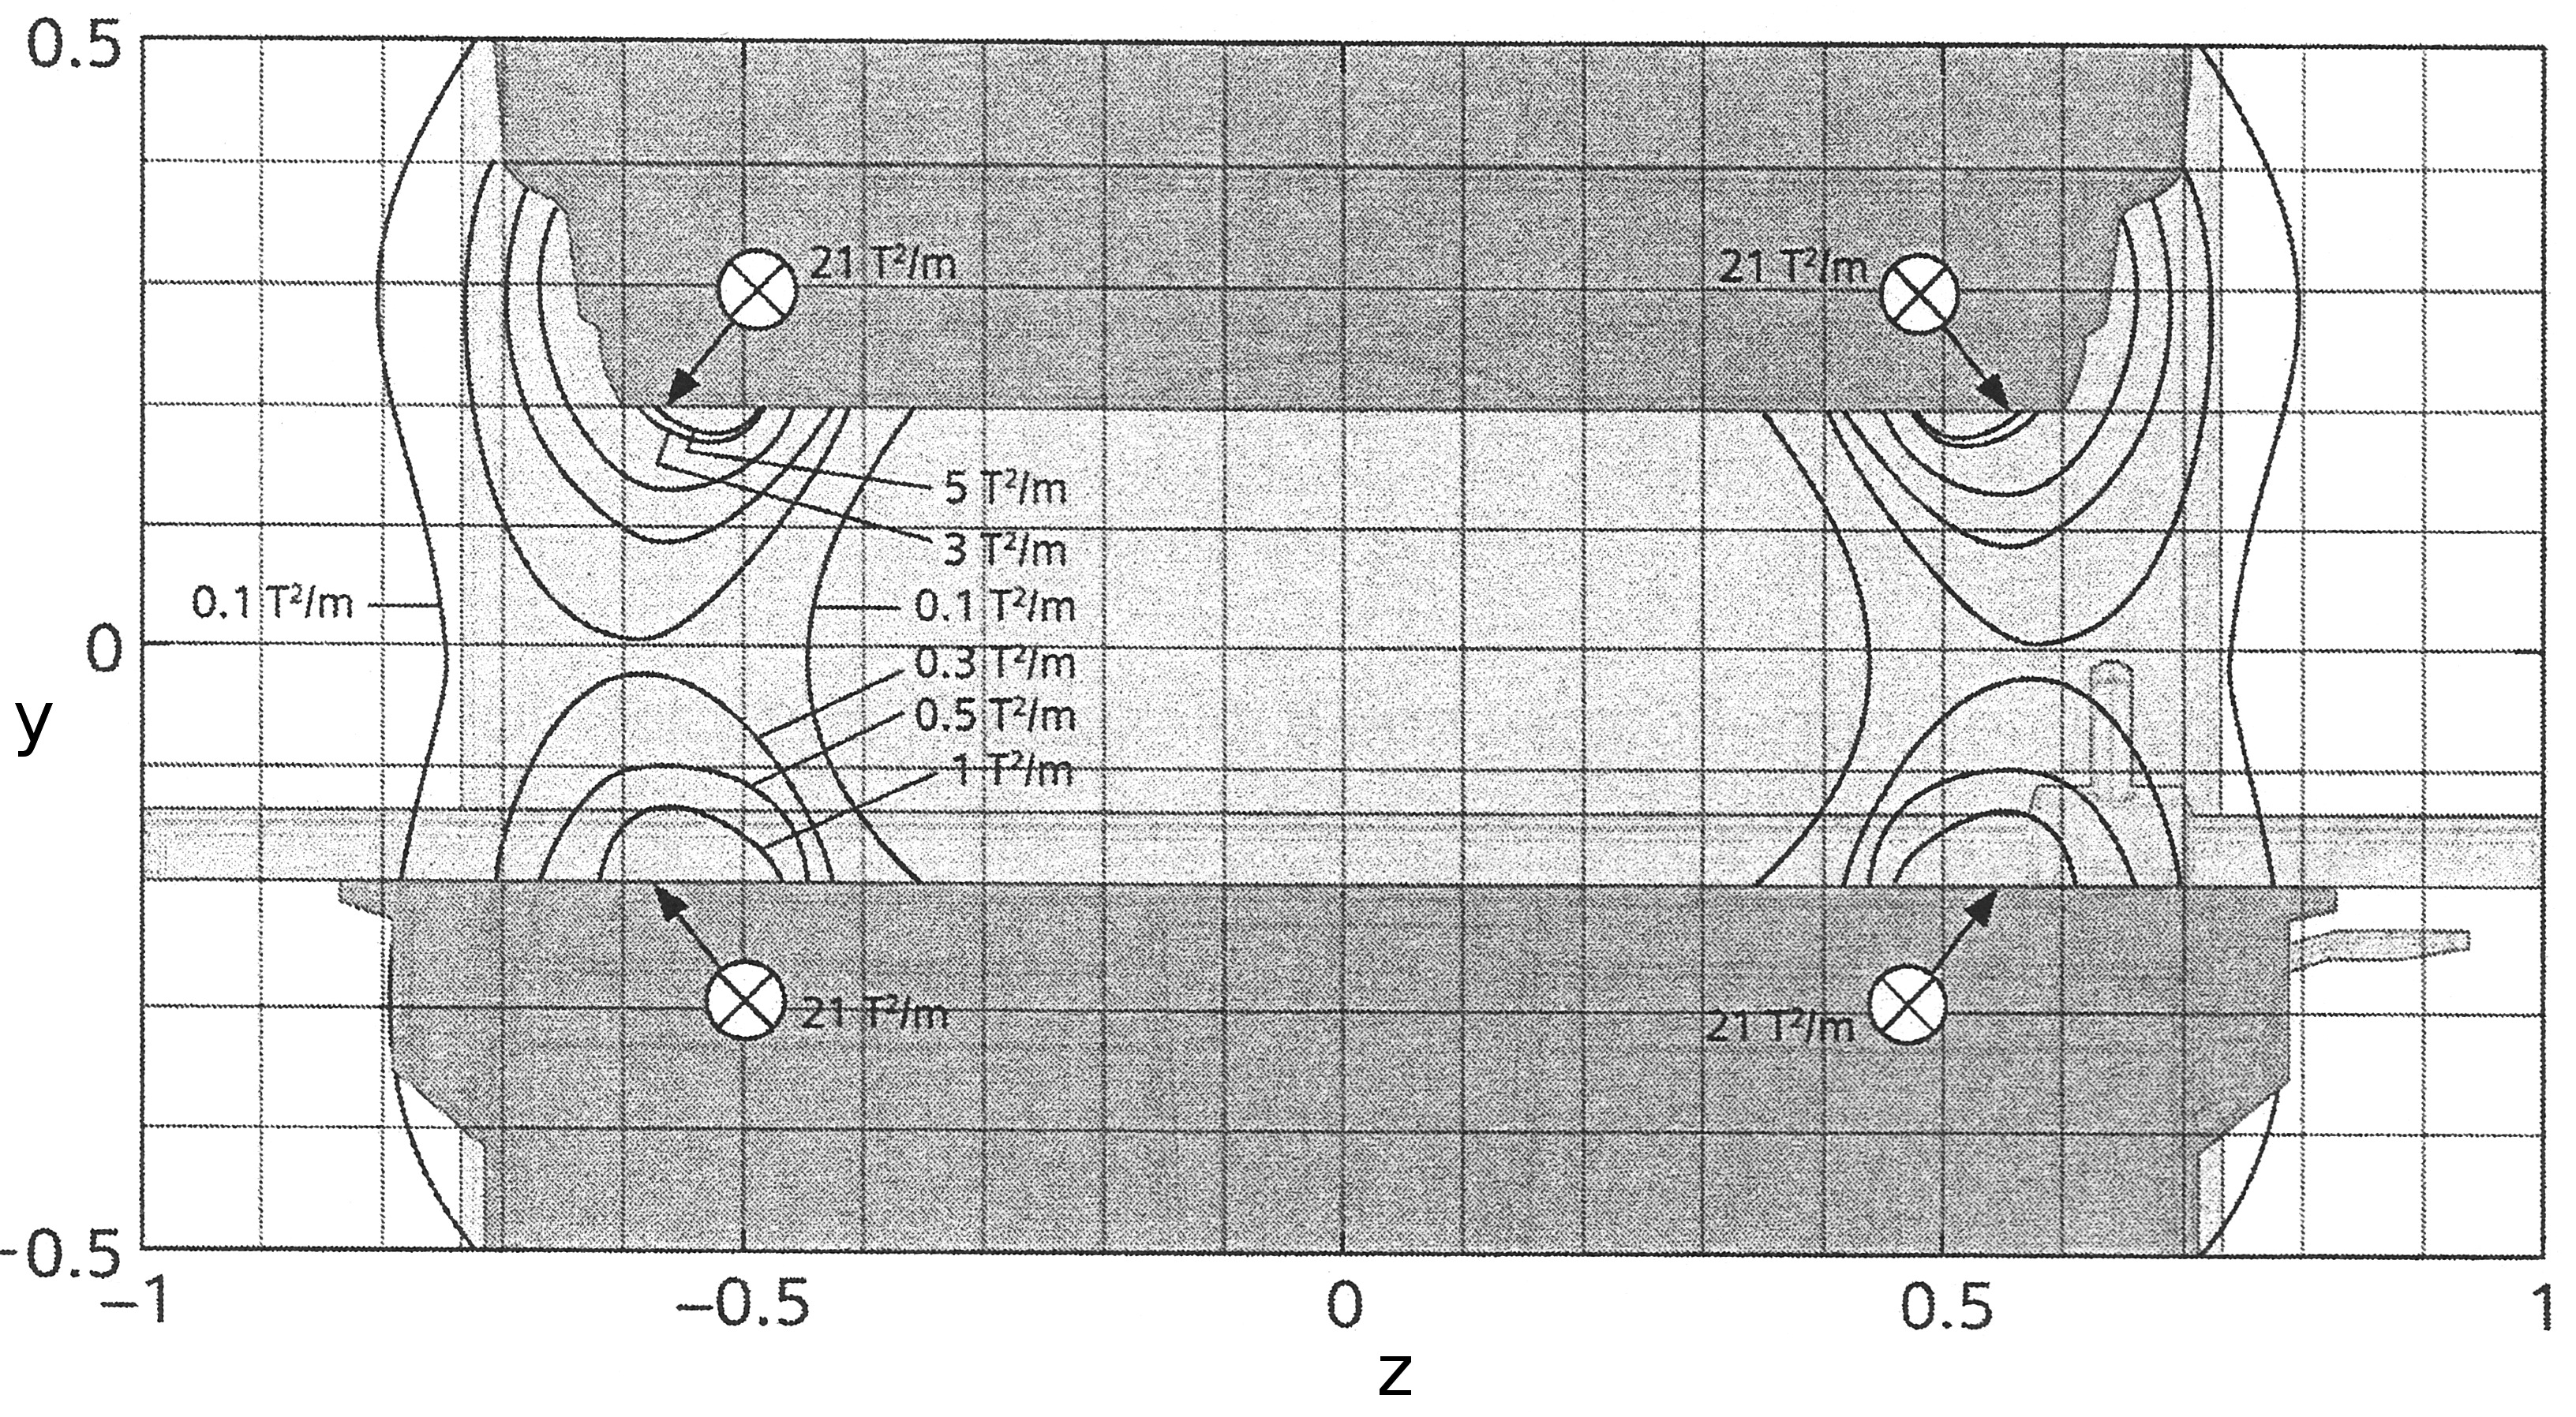
\includegraphics[scale=1]{scanner/scanner_gradient-front.jpg}
%    \caption{field gradient - front view (see fig. \ref{fig:scanner_front})}
%    \label{fig:gradient_front}
%  \end{subfigure}
%  \begin{subfigure}[b]{\textwidth}
%  	\centering
%    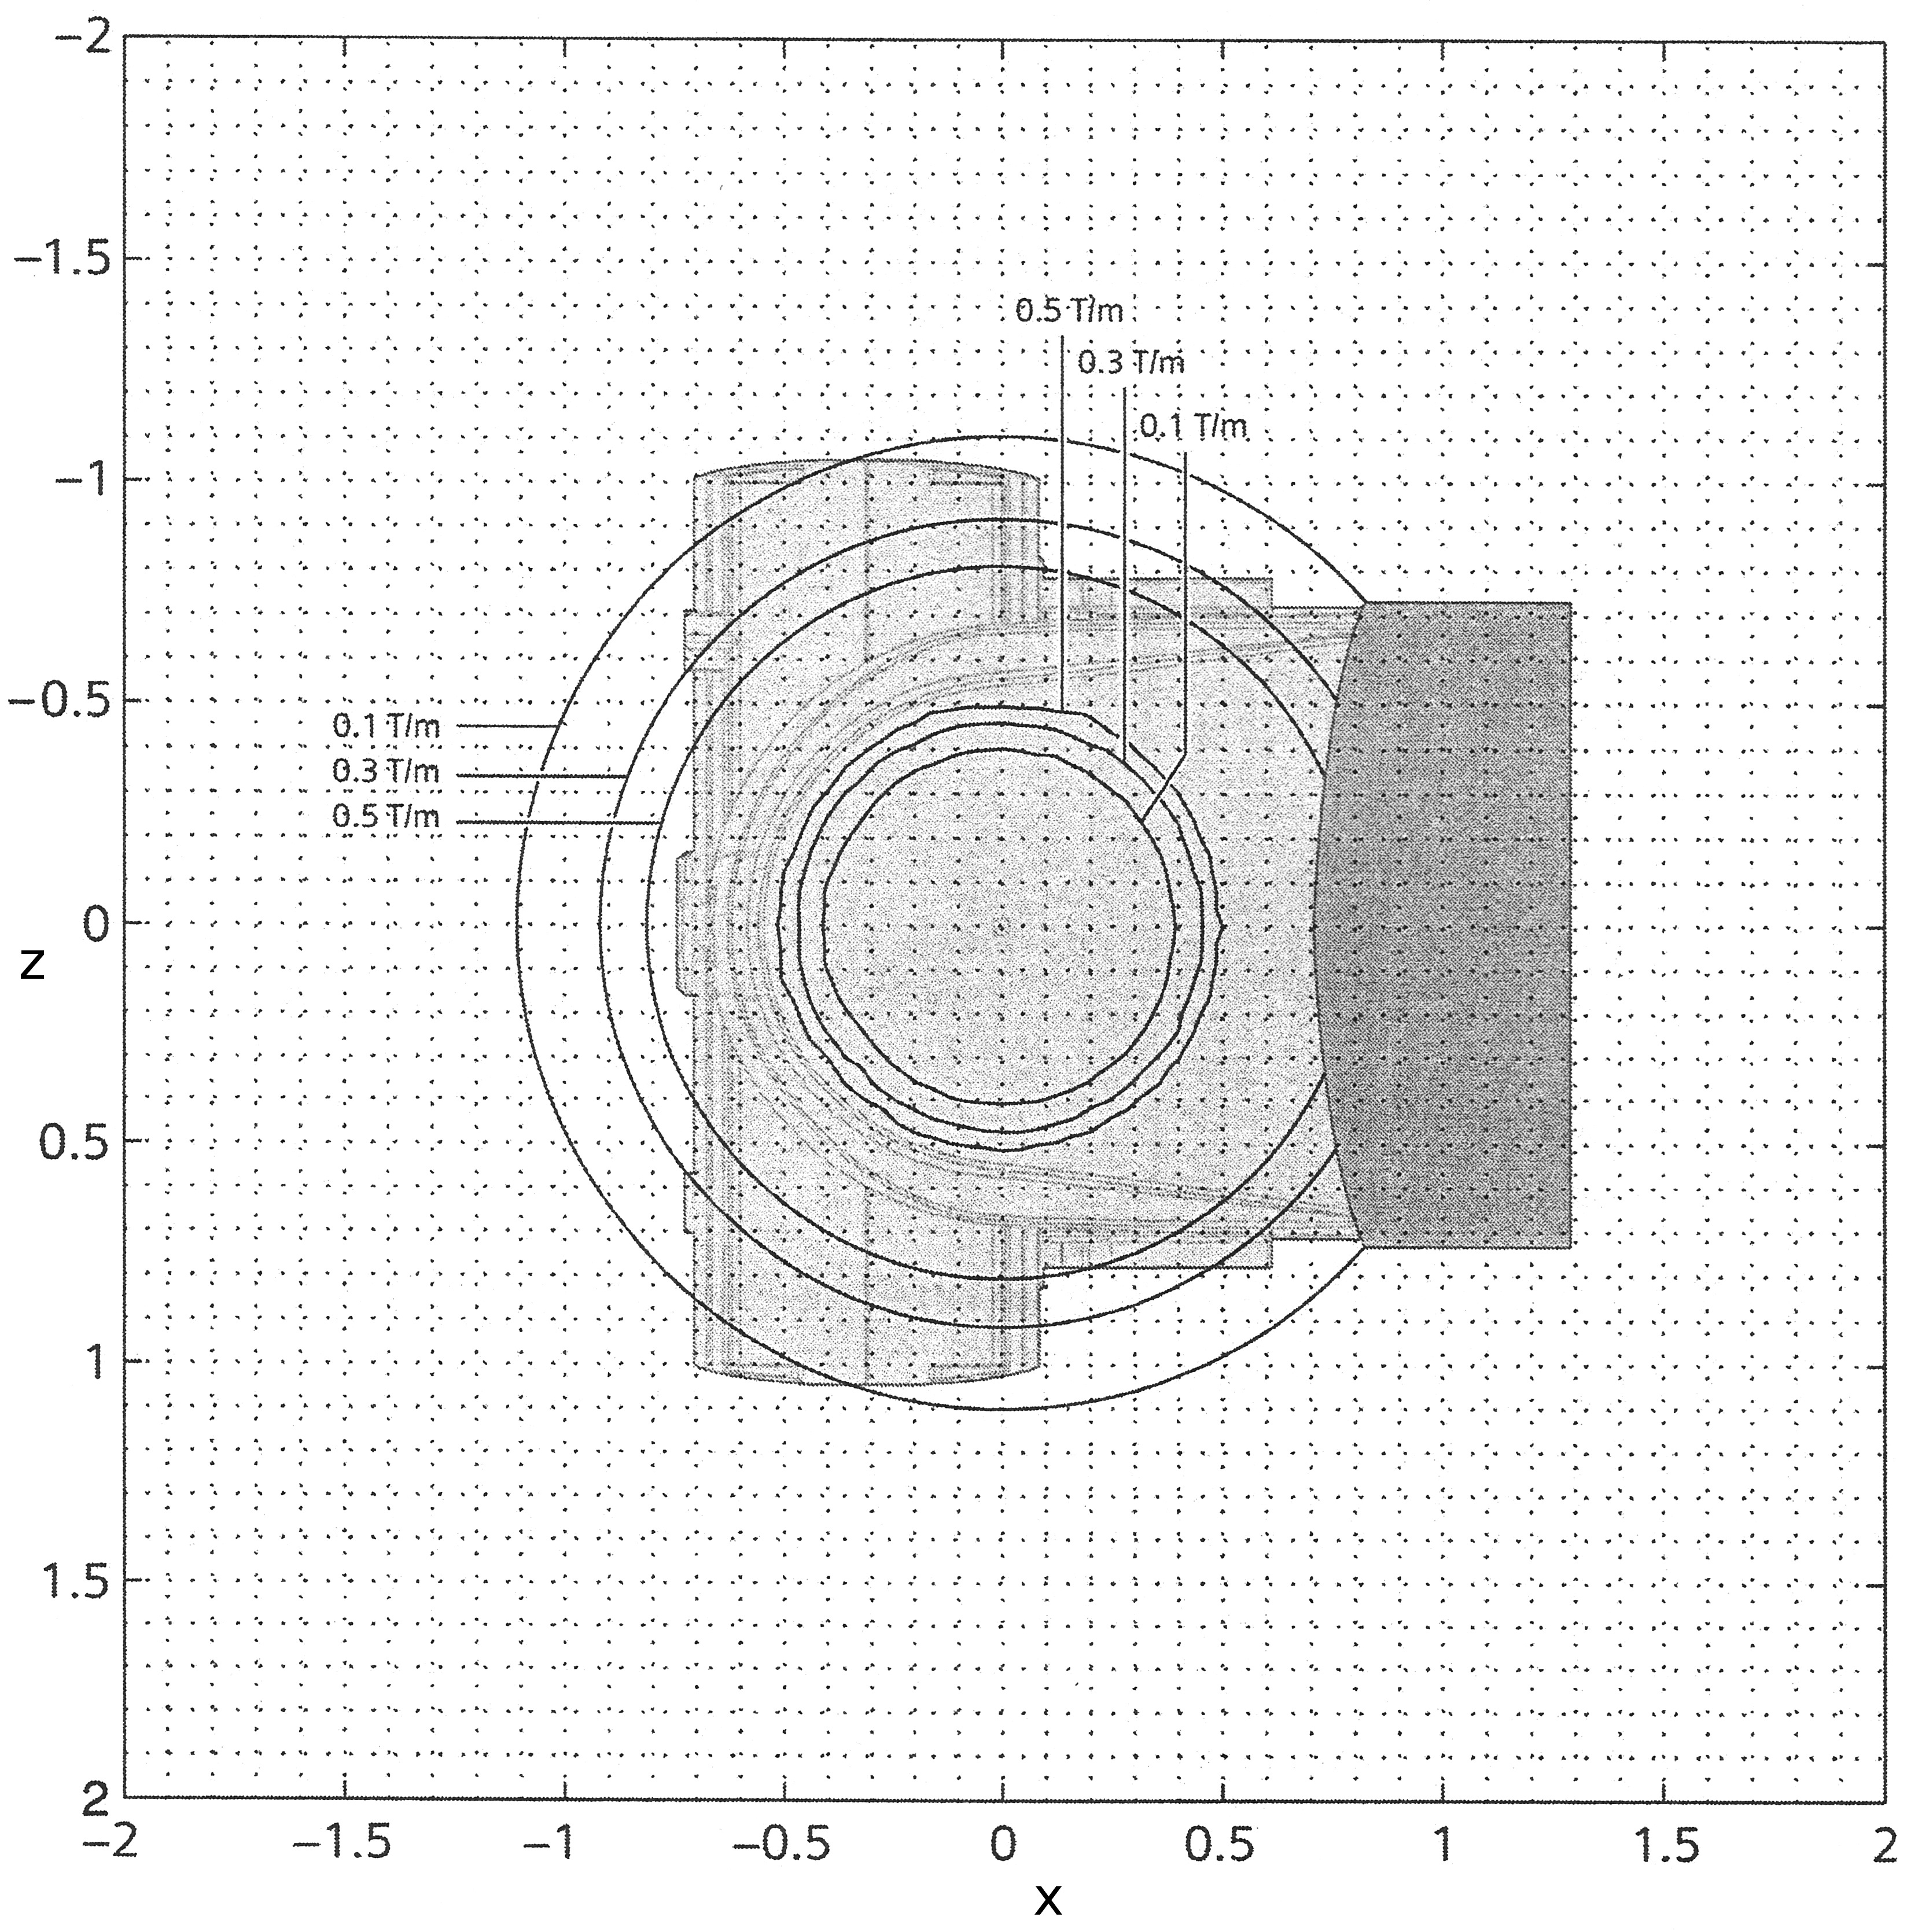
\includegraphics[scale=1]{scanner/scanner_gradient-top.jpg}
%    \caption{view along y-axis,\\ field gradient - top view (see fig. \ref{fig:scanner_top})}
%    \label{fig:gradient_top}
%  \end{subfigure}
%  \caption{Magnetom C! field gradient}
%  \label{fig:scanner}
%\end{figure}
%
%\begin{figure}[!htb]
%\centering
%  \begin{subfigure}[b]{\textwidth}
%    	\centering
%        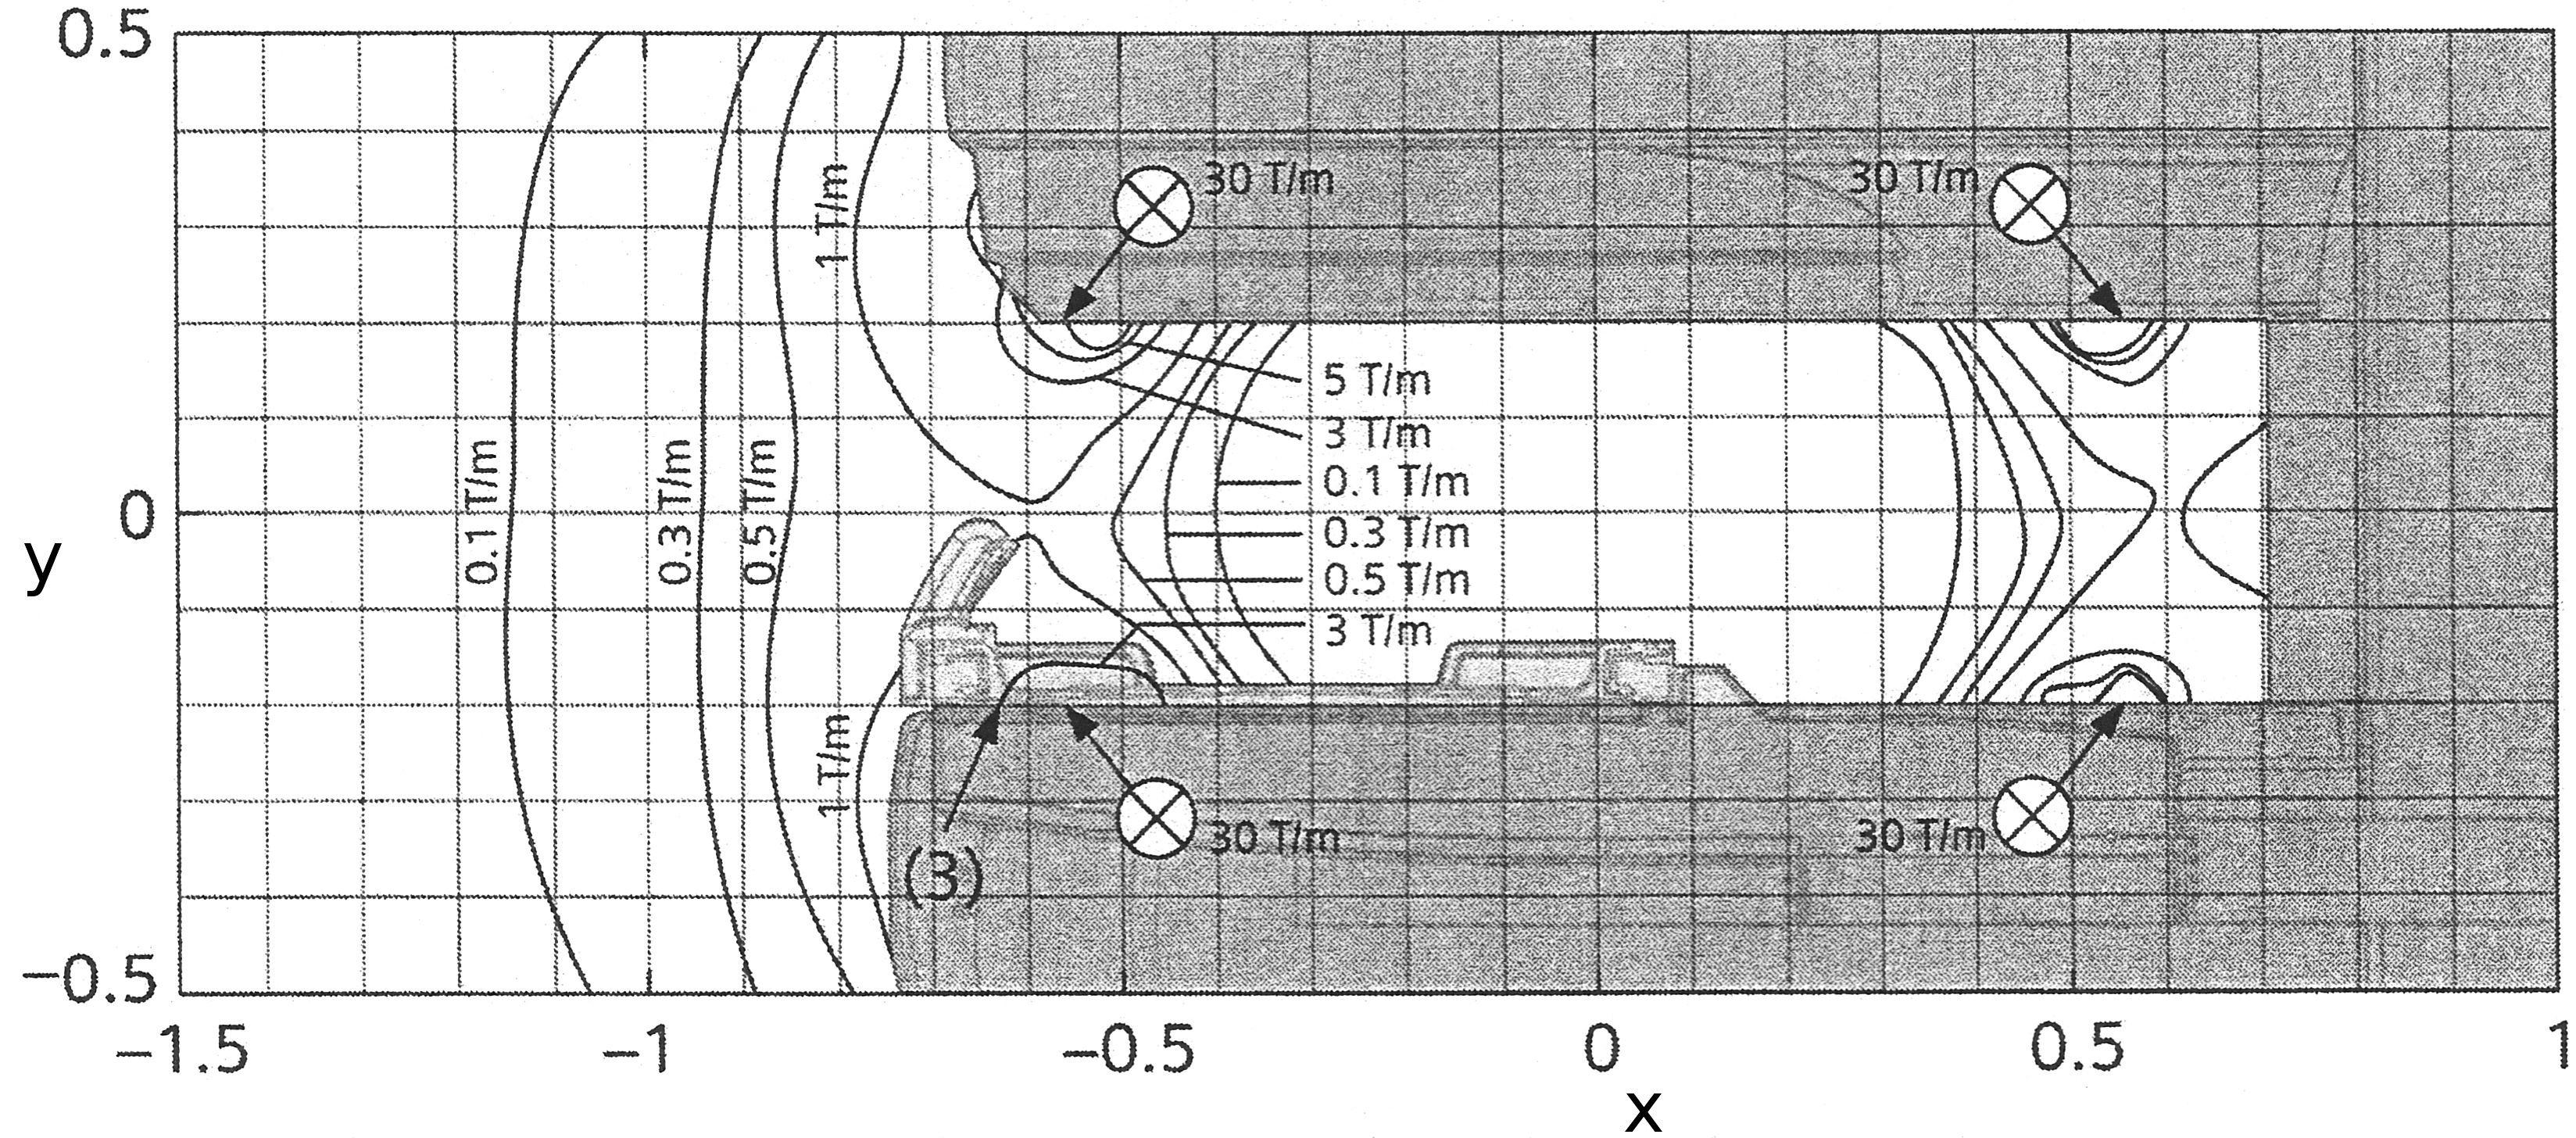
\includegraphics[scale=1]{scanner/scanner_gradient-side.jpg}
%        \caption{field gradient}
%        \label{fig:gradient_side}
%  \end{subfigure}
%  \begin{subfigure}[b]{\textwidth}
%  	\centering
%      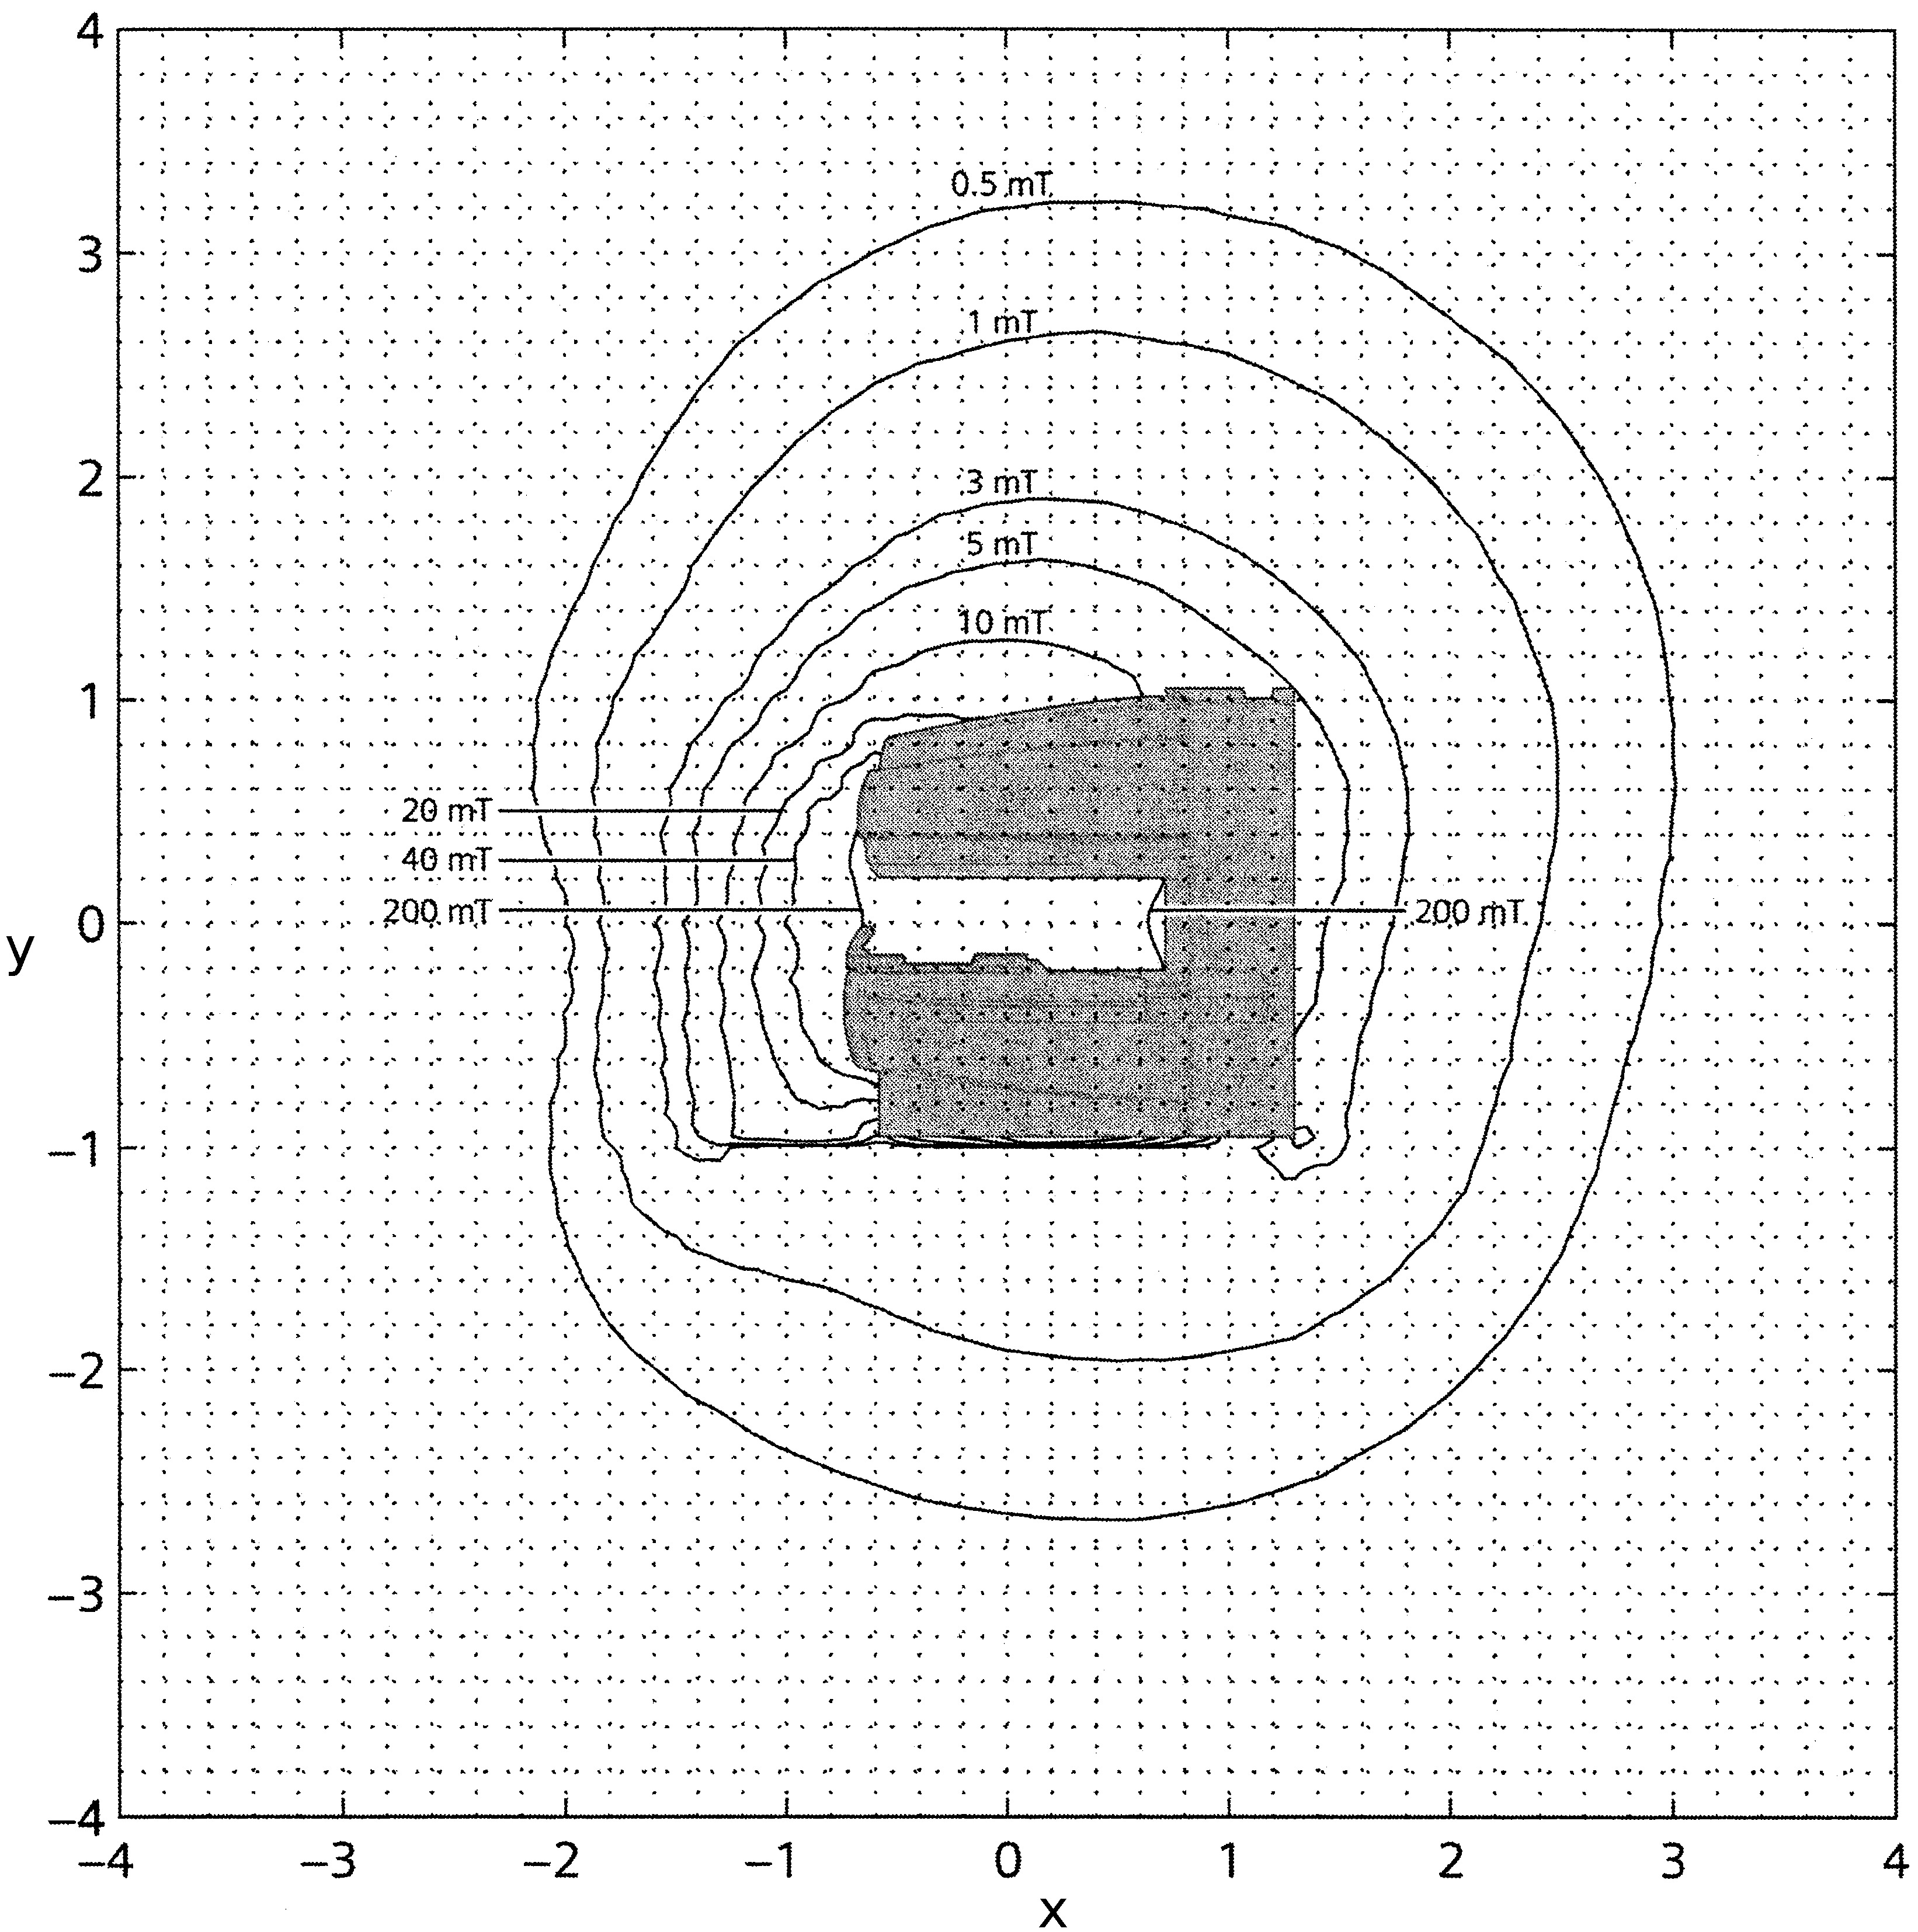
\includegraphics[scale=1]{scanner/scanner_field-strength.jpg}
%      \caption{field strength}
%    \label{fig:strength_side}
%  \end{subfigure}
%  \caption{Magnetom C! field gradient and strength - side view (see fig. \ref{fig:scanner_side})}
%  \label{fig:scanner_gradient}
%\end{figure}


\section{Custom build phantom}

To compare images from different scanners and asses occurring distortion, a rigid object with known dimensions is necessary.
Such a 'phantom' is often made from plastics containing a liquid.
The AKH's design is made up from an array of replaceable, fillable plastic rods.

\begin{figure}[!htb]
\centering
  \begin{subfigure}[b]{0.1\textwidth}
    
\includegraphics[scale=1]{slicer3D/full_phantom/sagittal_comparison_mr.png}
    \caption{MR}
    \label{fig:sagittal_comparison_mr}
  \end{subfigure}
  \begin{subfigure}[b]{0.1\textwidth}
    
\includegraphics[scale=1]{slicer3D/full_phantom/sagittal_comparison_ct_empty.png}
    \caption{CT}
    \label{fig:sagittal_comparison_ct_empty}
  \end{subfigure}
  \begin{subfigure}[b]{0.1\textwidth}
    
\includegraphics[scale=1]{slicer3D/full_phantom/sagittal_comparison_ct.png}
    \caption{CT}
    \label{fig:sagittal_comparison_ct}
  \end{subfigure}
  \caption{Comparison: MRI only shows liquid filling, CT also the plastic rod and pane (horizontal black bar crossing middle and right rod);\\ (\textbf{a:}) \textit{MRI} - filled rod, plastic not visible (field of view too small to show entire rod); (\textbf{b:}) \textit{CT} - empty rod, plastic visible; (\textbf{c:}) \textit{CT} - filled rod, plastic and filling visible}
  \label{fig:sagittal_comparison}
\end{figure}

\subsection{Frame and rods}

The phantom was build to fit the largest available rigid coil for the MRI scanner.
Three parallel acrylic glass panes in the shape of the coil serve as a frame for the plastic rods.
In the middle an empty area was reserved for an optional additional smaller phantom (not used for this work).
Figure \ref{fig:photo_ph3} shows a picture of the phantom. See also figure \ref{fig:axial_CT_pane} showing a CT image of one pane (with no rods inserted). \\
More than 300 plastic rods (length: 50cm, outer diameter: 8mm, inner diameter: 4mm, volume: approx. 6mL) could be placed in the phantom.
See figure \ref{fig:rod_schematic} for a schematic sketch of one rod.
The bottom part of each rod was sealed with a hot glued plastic plug, the top could be closed with a plastic screw.
Frame and rods were already build and assembled before the author started working on this project.

Additionally to the rods which would be used to assess the distortion, a number of vitamin-e pills were attached to the frame.
These pills are visible in both CT and MRI images were used to align both scans.
This way there is another way of checking the alignment in addition to the rods.
\todo{show picture/CT-/MRI-scan of vitamin-e pills??}


\begin{figure}[!bp]
\centering
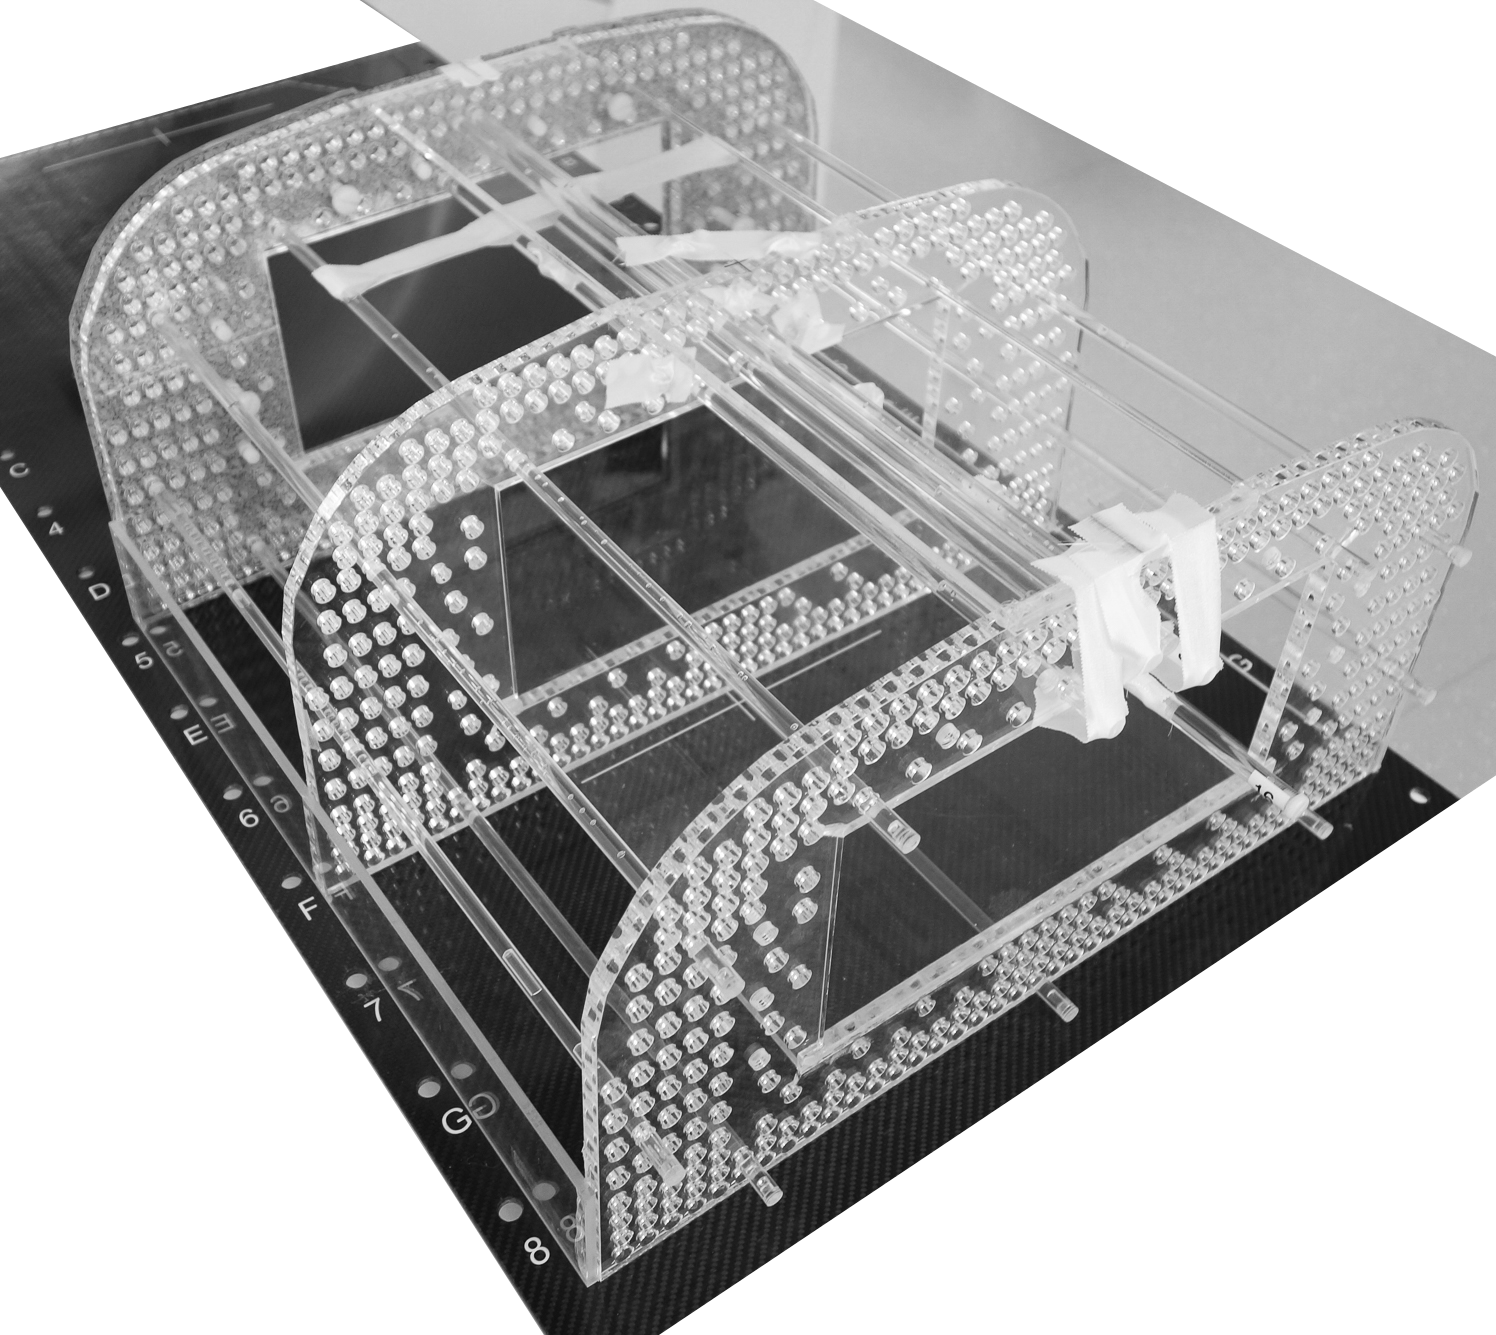
\includegraphics[width=\textwidth]{photo/ph3_CT-scanner.png}
\caption{Picture of phantom on CT desk}
\label{fig:photo_ph3}
\end{figure}

\begin{figure}[!tbp]
\centering
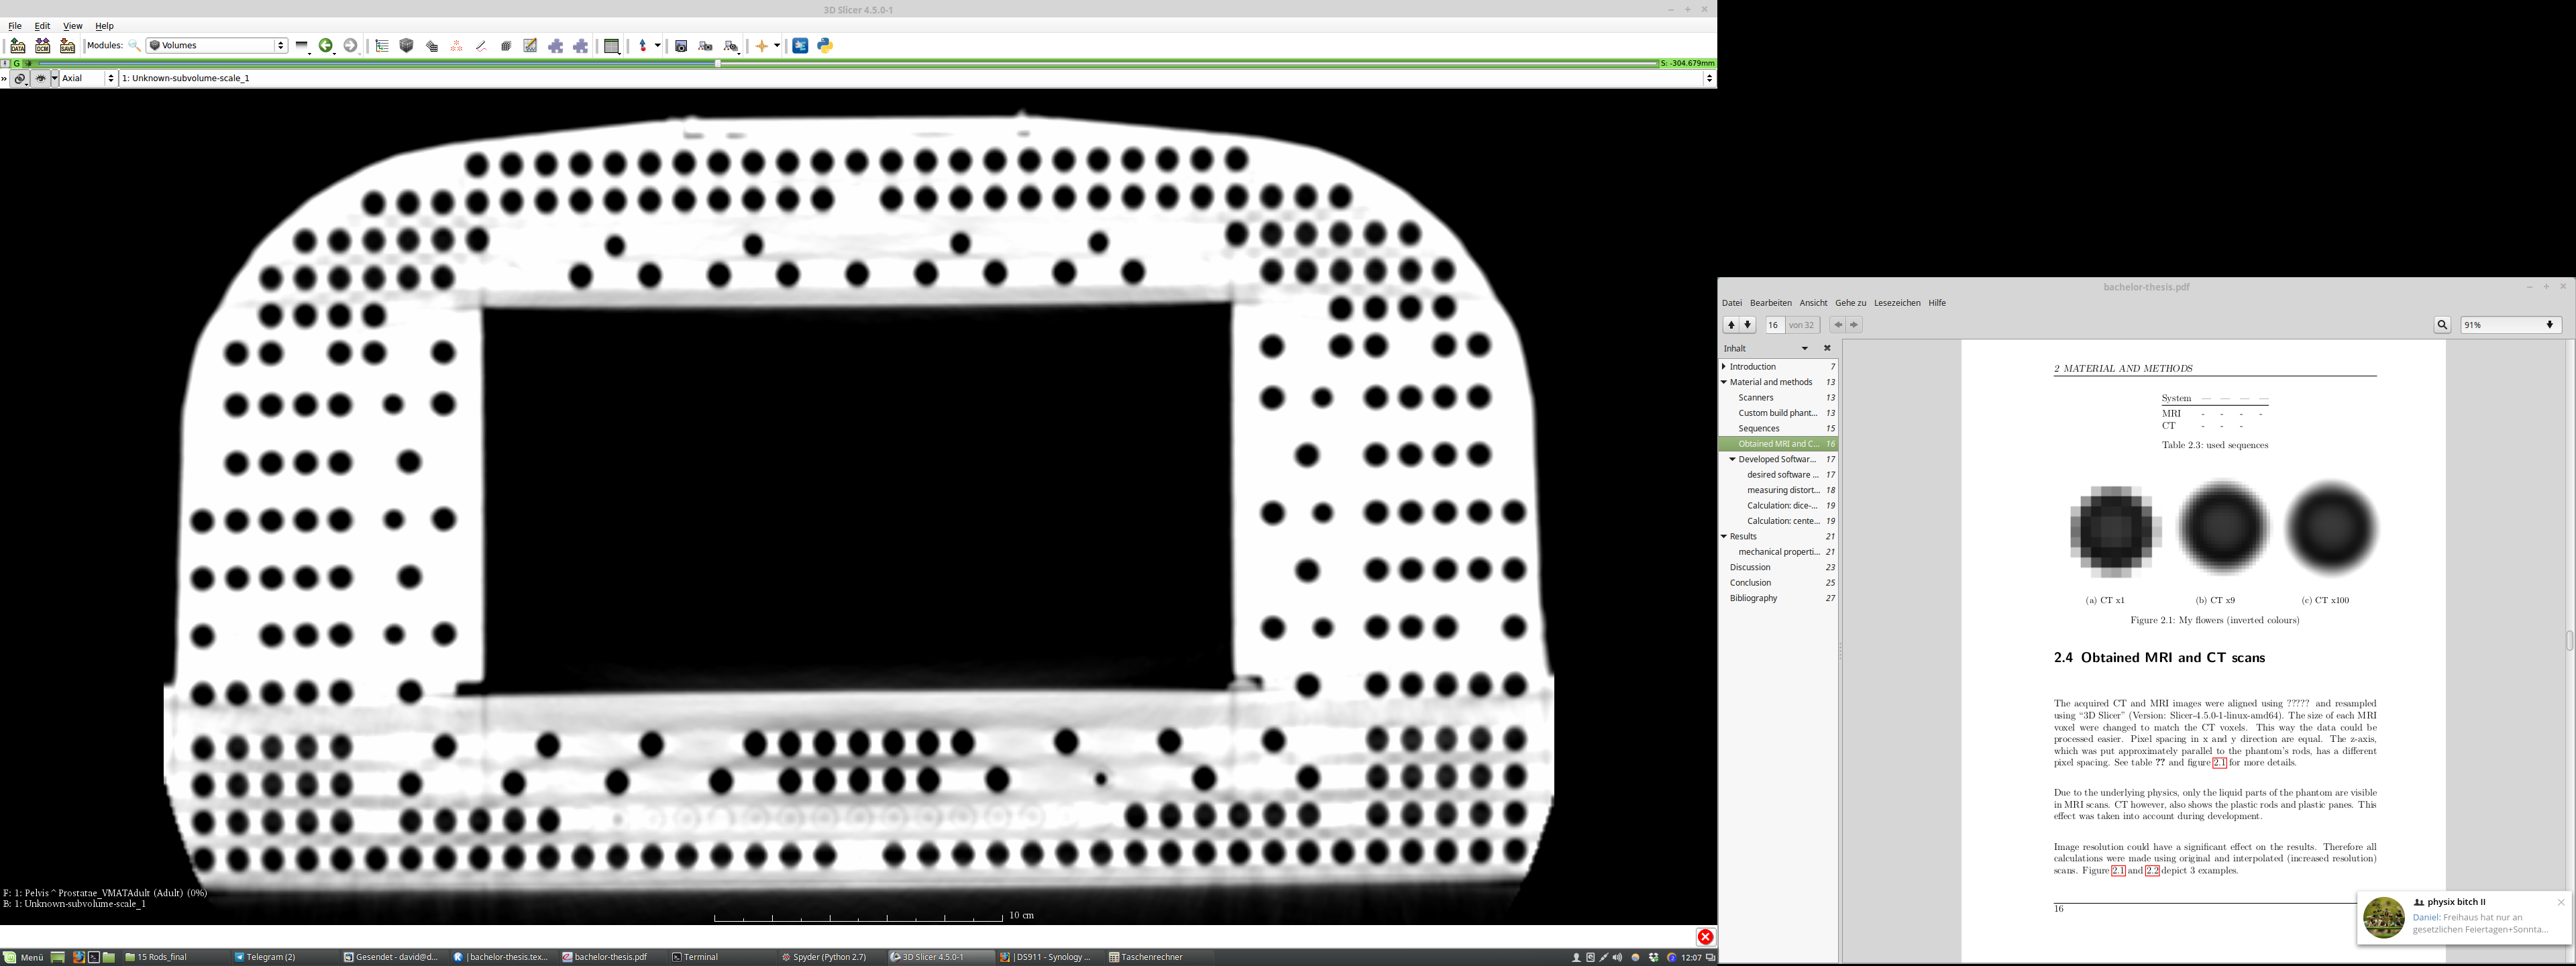
\includegraphics[width=\textwidth]{slicer3D/full_phantom/axial_CT_pane.png}
\caption{plastic pane, no rods inserted}
\label{fig:axial_CT_pane}
\end{figure}

\begin{figure}[!tbp]
\centering
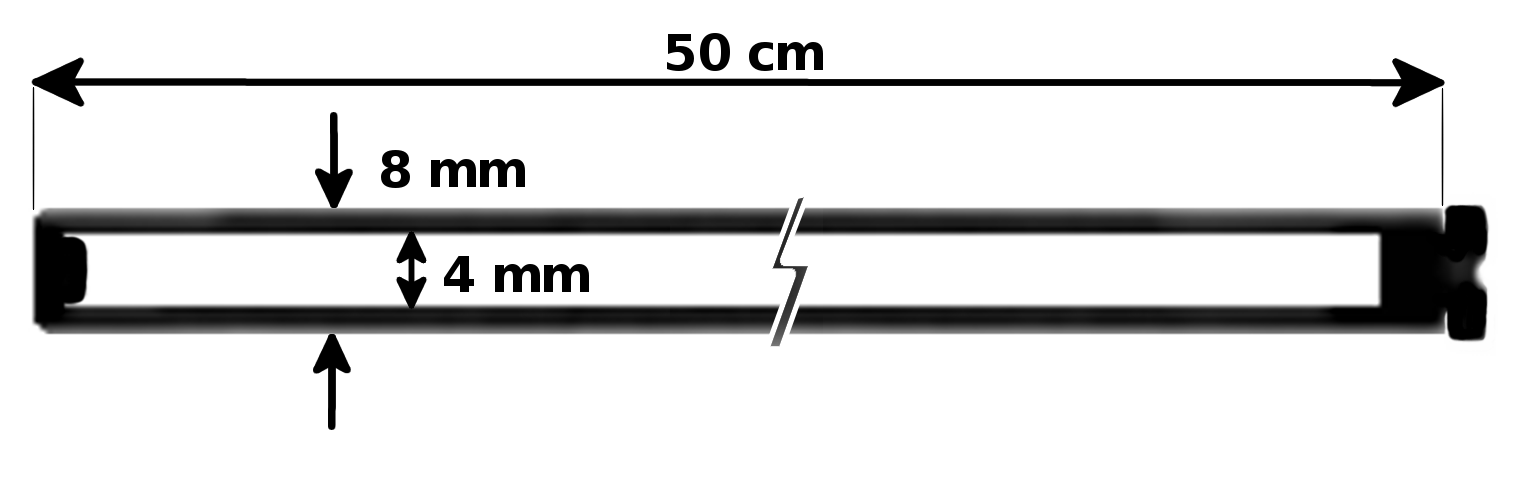
\includegraphics[width=0.8\textwidth]{slicer3D/full_phantom/rod_schematic.png}
\caption{empty plastic rod, schematic (not true proportions); }
\label{fig:rod_schematic}
\end{figure}

\clearpage

\subsection{Rod fillings}

For this study 17 different liquids were produced to be tested as possible fillings.
They are listed in Table \ref{tab:solutions}.


\begin{table}[!hbt]
\centering
\begin{tabular}{@{}l|rrrrrr@{}}
No.   & $NaCl$   & $CuSO_4\cdot5H_2O$          & Soap & Ascorbic Acid & Agar & Primovist [volume-\%]\\
\toprule
\#1  &             &                   &      &               &           &		\\
\#2  & 3.6         & 1.96              &      &               &           &		\\
\#3  & 3.6         & 3.92              &      &               &           &		\\
\#4  & 3.6         & 19.6              &      &               &           &		\\
\#5  & 3.6         & 1.96              & 1    &               &           &		\\
\#6  & 3.6         & 1.96              & 5    &               &           &		\\
\#7  & 3.6         & 1.96              & 20   &               &           &		\\
\#8  & 3.6         & 1.96              &      & 0.36          &           &		\\
\#9  & 3.6         & 1.96              &      & 3.6           &           &		\\
\#10 & 3.6         & 1.96              &      & 36            &           &		\\
\#11 & 3.6         &                   &      &               &           & 0.1\%	\\
\#12 & 3.6         &                   &      &               &           & 1\%		\\
\#13 & 3.6         &                   &      &               &           & 10\%	\\
\#14 & 3.6         & 1.96              &      &               &  0.5      &		\\
\#15 & 3.6         & 1.96              &      &               &   20      &		\\
\midrule
\#16 & \multicolumn{2}{r}{Motor Oil:}   & \multicolumn{4}{l}{\textit{Castrol Power1}}      \\
\#17 & \multicolumn{2}{r}{Silicon Oil:} & \multicolumn{4}{l}{\textit{Charge: 15HLVY023}}   \\ \bottomrule
\end{tabular}
\caption{composition of tested solutions\\(components in $g/L$; exception: Primovist in volume-\%)}
\label{tab:solutions}
\end{table}

\newpage
\begin{enumerate}[label=\textbf{\#\arabic*}]
 \item \textit{distilled water}
 \item $NaCl$ + $CuSO_4\cdot5H_2O$
 \item increased concentration of $CuSO_4\cdot5H_2O$
 \item further increased concentration of $CuSO_4\cdot5H_2O$
 \item generic washing-up \textit{soap} added to \textbf{\#2}
 \item increased \textit{soap} concentration
 \item further increased \textit{soap} concentration
 \item \textit{ascorbic acid} added to \textbf{\#2}
 \item increased \textit{ascorbic acid} concentration
 \item further increased \textit{ascorbic acid} concentration
 \item \textit{Primovist}
 \item increased amount of \textit{Primovist}
 \item further increased amount of \textit{Primovist}
 \item \textit{agar}
 \item increased \textit{agar} concentration
 \item synthetic motor oil
 \item silicon oil
\end{enumerate}

Being closed at one end and having a capillary shape (small diameter) makes it impossible to fill the rods by simply pouring the liquid through the opening.
Instead of adding the fluid at the top, it has to be injected starting at the bottom.
This way the contained air would be pushed out by the injected liquid through the opening at the top.
A thin plastic tube was inserted and used for injection, leaving enough room for the gas to escape.
Between injections of different liquids, the tube was flushed with \textbf{\#1} (distilled water) or \textbf{\#2} (main component of most solutions).

In order to minimise the amount of gas dissolved, the liquids were brought to boil shortly before injecting. Gas solubility generally decreases with rising temperature \cite{Henry1803, Sander2015}.
After injecting the solution in the rods, they were left to cool down.
Before closing, the rods were topped up completely (no trapped air bubbles).
The oil based liquids, \textbf{\#16} and \textbf{\#17}, were not brought to boil.


\section{Sequences}
\todo{elaborate!}
Following the suggestions given in the Report of AAPM MR Subcommittee TG1 "MR Acceptance Testing and
Quality Control" \cite{Jackson2009}, T1 weighted sequences were chosen to evaluate the possible solutions. (Table \ref{tab:settings})

\begin{table}[h]
\centering
\begin{tabular}{@{}lllll@{}}
System & ---  & --- &  --- & --- \\
\toprule
MRI    & -   & -   & -   & -    \\
CT     & -   & -   & -   &
\end{tabular}
\caption{used sequences}
\label{tab:settings}
\end{table}

\section{Developed software tool}
% conda create --name snowflakes python=2.7 SimpleITK Spyder
% source activate snowflakes
% spyder

In order to asses the distortion of the MRI scanner, a tool was programmed.
It is written in Python 2.7 and uses the \textit{SimpleITK} package to read and process \textit{DICOM} ("\textit{Digital Imaging and Communications in Medicine}") files. \cite{Python, DICOM}
\textit{SimpleITK} is a object-oriented "C++ library with wrappers for Python, Java, CSharp, R, Tcl and Ruby". \cite{SimpleITK, SimpleITK_started} It's versatility is one of the reasons why this approach was favoured.
It is a simplified layer built on top of the National Library of Medicine Insight Segmentation and Registration Toolkit (ITK). SimpleITK is also used by Applications like \textit{3D Slicer} , a "free and open source software package for
visualisation and medical image computing". \cite{3DSlicer, Kikinis2012} For this work 3D Slicer was used to crop and resample images, quickly read values, and visualise the results.
Documentation and code examples of SimpleITK can be found at \cite{InsightSoftwareConsortium, Kyriakou-SimpleITK}
An alternative way to handle DICOM data in Python would be Pydicom. \cite{Pydicom, Kyriakou-Pydicom-VTK} 

This is an extensive list of python packages used to process data after using 3D Slicer:
\begin{itemize}
 \item SimpleITK
 \item numpy
 \item scipy
 \item matplotlib.pyplot \cite{Hunter2007}
 \item skimage.draw
 \item datetime
 \item os
\end{itemize}

\subsection{Pre-processing MRI and CT scans}
\label{sec:prep}

% what application used to align CT and MRI
Prior to analysing their data, the scans had to be prepared.
Figure \ref{fig:data_prep} gives an impression how the steps performed affected the data.

\begin{enumerate}[label=\textbf{Step \arabic*}]
\item After loading the CT and MRI scan into \textit{MIRADA}, they were aligned using the vitamin-e pills, yielding maximum overlap in the centre of the image.
\item Next, as the MRI image had a lower resolution than the CT scan, the MRI scan was resampled.
Its voxel's size were changed to match the CT voxels and both scans exported.
\item Both layers (MRI and CT) were loaded into \textit{3D Slicer} (Versions: Slicer-4.5.0-1-linux-amd64, Slicer-4.6.2-win-amd64)
\item Its module 'annotations' was used to set a new region of interest (ROI) to include only a single rod.
\item With the module called 'crop volume' (setting: voxel based cropping) the scans were reduced to show only the selected ROI.
\item Using the module 'resample scalar volume' a number of interpolated (setting: 'bspline') higher resolution pairs (CT/MRI) were created.
\item All new pairs and the cropped original CT/MRI pair were exported with 'create a dicom series' and saved in a separate folder each.
\end{enumerate}

\begin{figure}[!tbp]
\centering
\includegraphics[width=0.8\textwidth]{algorithm/data_prep.jpg}
\caption{Steps performed before analysing data with script}
\label{fig:data_prep}
\end{figure}

After this procedure a number of pairs based on the original CT and MRI were available, all of which had the same number of slices along the z-axis parallel to the phantom's rods.
They only differ in the number of pixels making up each slice, their resolution varying from the original up to a hundred times finer.
Each pair (CT/MRI) has the same pixel spacing (and resolution) in x and y direction.
See table \ref{tab:spacing} for more details.
Figure \ref{fig:resample} depicts 3 CT/MRI scans of a single rod (axial) with different resolutions.
"x1" stands for the original CT scan resolution (MRI resampled to match).
"x4" is a resolution caused by 1 pixel being split in 4 smaller pixels, "x9" in 9, and so on and so forth.
For better visibility, images shown as figures in this work are printed with inverted colours.
Dark pixels have a high density/intensity value, white pixels are equivalent to air (low density/intensity).

\begin{table}[!htb]
\centering
\begin{tabular}{l|l|l|l}
resample factor  & z (not affected) &  y (same as x) & x \\
\toprule
x1     & 0.60 & 0.98	& 0.98	\\
x4     & 0.60 & 0.49	& 0.49	\\
x9     & 0.60 & 0.33	& 0.33	\\
% x16    & 0.60 & 0.244	& 0.24	\\
x25    & 0.60 & 0.2 	& 0.2	\\
x100   & 0.60 & 0.2 	& 0.1
\end{tabular}
\caption{pixel Spacing (rounded values) [$mm$]}
\label{tab:spacing}
\end{table}


\begin{figure}[!thb]
  \begin{subfigure}[b]{0.32\textwidth}
    
\includegraphics[scale=.11]{slicer3D/profiles/CT_x1.png}
    \caption{CT x1}
    \label{fig:CT_x1}
  \end{subfigure}
  \hfill
  \begin{subfigure}[b]{0.32\textwidth}
    
\includegraphics[scale=.11]{slicer3D/profiles/CT_x9.png}
    \caption{CT x9}
    \label{fig:CT_x9}
  \end{subfigure}
    \hfill
  \begin{subfigure}[b]{0.32\textwidth}
    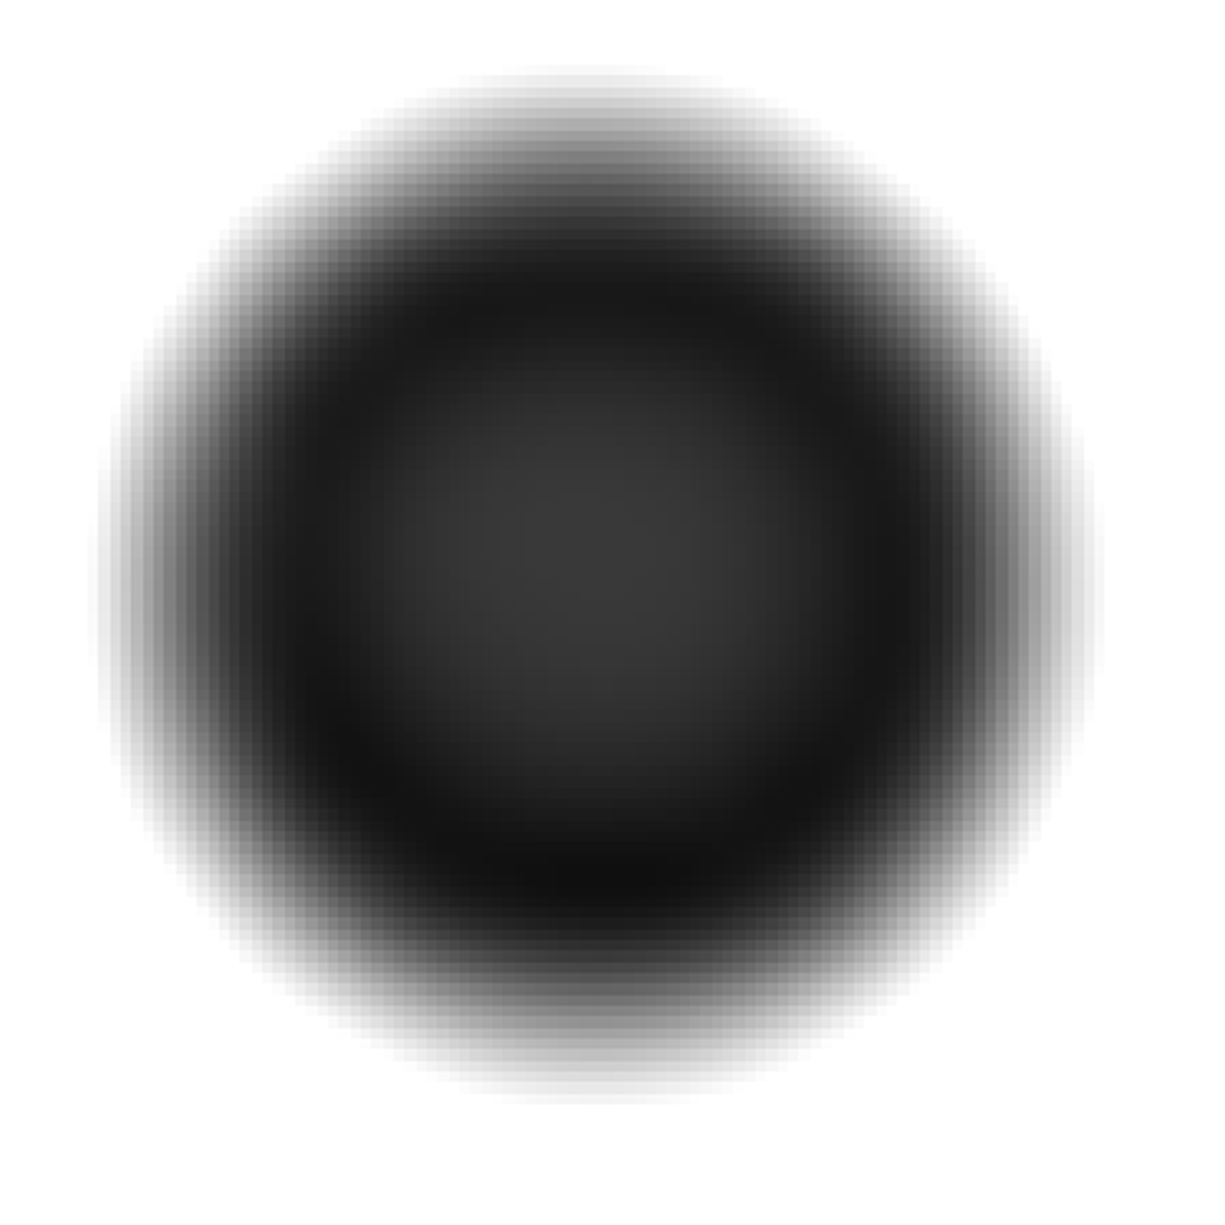
\includegraphics[scale=.11]{slicer3D/profiles/CT_x100.png}
    \caption{CT x100}
    \label{fig:CT_x100}
  \end{subfigure}
  \begin{subfigure}[b]{0.32\textwidth}
    
\includegraphics[scale=.11]{slicer3D/profiles/MR_x1.png}
    \caption{MRI x1}
    \label{fig:MRI_x1}
  \end{subfigure}
  \hfill
  \begin{subfigure}[b]{0.32\textwidth}
    
\includegraphics[scale=.11]{slicer3D/profiles/MR_x9.png}
    \caption{MRI x9}
    \label{fig:MRI_x9}
  \end{subfigure}
    \hfill
  \begin{subfigure}[b]{0.32\textwidth}
    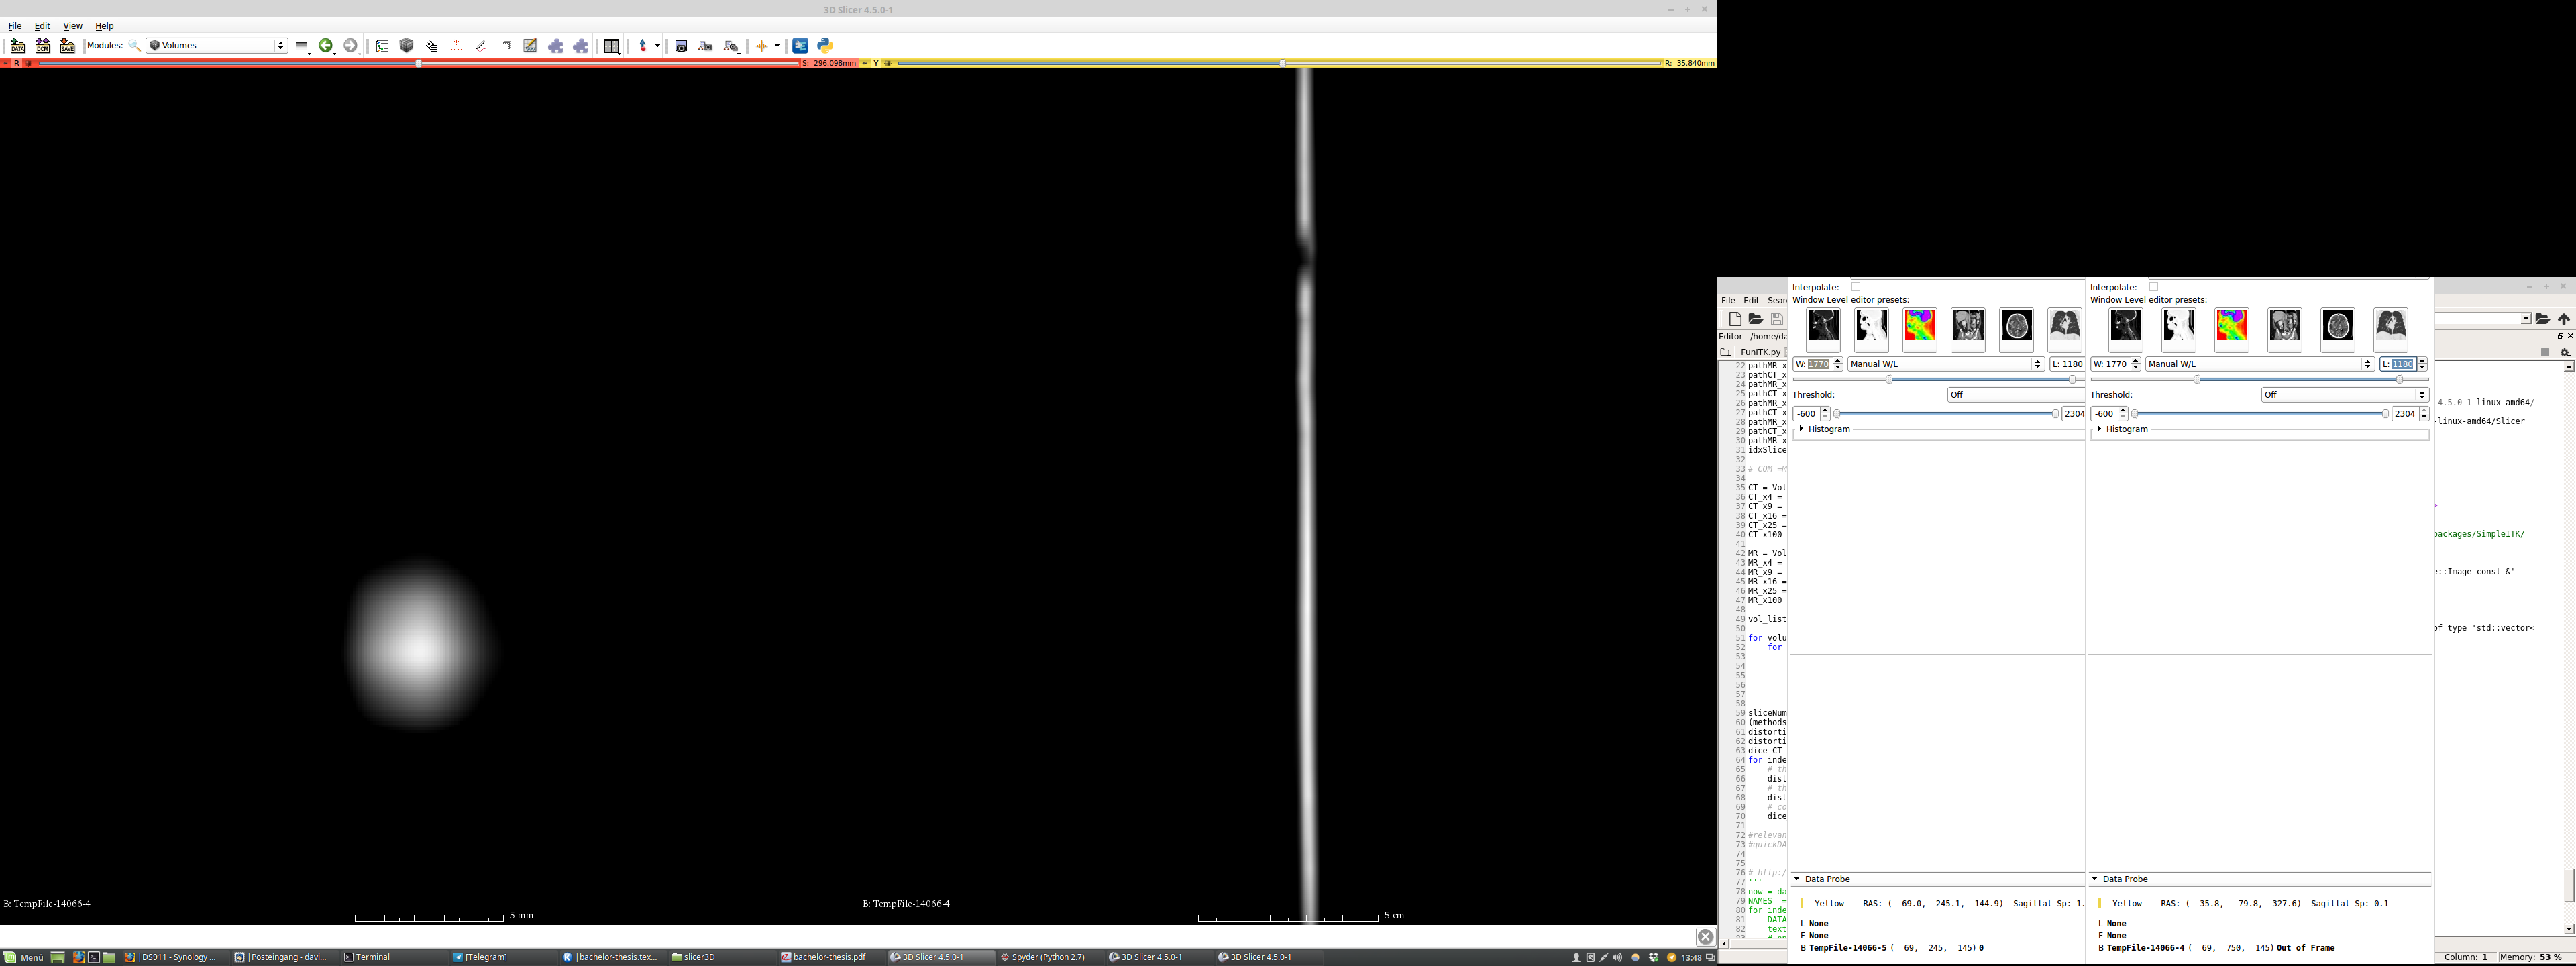
\includegraphics[scale=.11]{slicer3D/profiles/MR_x100.png}
    \caption{MRI x100}
    \label{fig:MRI_x100}
  \end{subfigure}
  \caption{CT/MRI: axial image of single rod, filling \#5  (inverted colours)}
  \label{fig:resample}
\end{figure}
\clearpage


\subsection{Capabilities}

The developed software tool is not able to automatically detect individual rods shown in a CT or MRI scan.
Instead the acquired 3D images have to be cropped to depict only a single rod (see section \ref{sec:prep})

The python script can be used to:
\begin{itemize}
 \item de-noise the image data
 \item separate bright areas which are not connected ('masking' might be used as future method to automatically detect individual rods)
 \item find and mark slices which show irregularities
 \item calculate the centroid coordinates along the rod
 \item measure the local distortion described by the
  \subitem location shift ( \textbf{"warp"})
  \subitem dice coefficient ( \textbf{"DC"} equivalent to roundness)
 \item visualise individual rod slices
 \item plot the average/peak brightness, warp, or DC along the rod
 \item write the warp and DC values for each slice in a combined ".txt" file
 \item export a rod shaped scan where the pixel values reflect the distortion occurring in each slice instead of their brightness as a ".mha" file (useful for visualisation)
\end{itemize}

\subsubsection{Measuring distortion}

Since the rods have a cylindrical shape, distortion can only be assessed in radial direction.
The z-coordinate is parallel to the rods, x and y are radial.
Ideally, each slice (z = const.) should depict the bright circular profile of the liquid (and plastic rod in CT) surrounded by black pixels (air).
\\
Two phenomena were chosen to reflect the amount of distortion occurring in each slice of the MRI scans.
The distance which the rod appears to be shifted in the MRI slice compared to the CT slice is referred to as \textbf{"warp"}.
The rod's deformation (deviation from circular profile) is described using the dice-coefficient \textbf{"DC"} (also known as Sorensen-Index).

\subsubsection{Detection of irregularities}

When the script loads the image data it also asks for a reference slice.
This reference slice will be used to decide if and which other slices might show irregularities, for example air bubbles, markers, or plastic panes.
It is the user's responsibility to chose one that is free from any such objects as reference slice.
Ideally, it is located near the iso-centre and has a brightness that is representative for the whole image.

To decide whether a slice is "irregular", it's average brightness will be compared to the reference slice's.
If the difference exceeds a certain value, the slice will be marked as irregular and consequently won't be used to calculate its DC or COM.
Instead these and the values describing the location shift will be set to "$-1$", indicating that no meaningful value could be obtained.
As the value referred to as \textit{warpMagnitude} and the DC are defined to be positive numbers, these are easily understood to be invalid, indicating that the particular slice was marked as "irregular".
The values representing x- and y-shift, on the other hand, are allowed to be negative or positive.
To be consistent with the other calculated numbers, they are still set to "$-1$".
The other values associated with the slice and discontinuities (values jumping to exactly "-1") where they meet neighbouring "regular" slices also indicate that this value is not representing the true distortion.

\subsection{Calculation: dice-coefficient (DC)}

The dice-coefficient was chosen as indicator for the deviation from a circular profile.
This value was calculated for the CT and MRI scans in every slice and saved in an array.
The DC ranges from 0 to 1.
A value of 1 indicates a perfect circular shape.
A low DC, on the other hand, means the shape differs greatly from a circle and could be caused by many things such as:
little overlap (e.g. a ring or crescent shape); a very dark image hindering delineation of rod from background; a small circle with a radius close to a only a few pixels.

The dice coefficient or Sorensen index \cite{MedPy_dc-doc} is defined as:

\begin{align}
DC = \frac{2 |A \, \cap \, B|}{|A| + |B|}
\end{align}

The implementation into python is based on the open source python package "Medpy". \cite{MedPy} A part of it's module called "metric" was adapted. \cite{MedPy_dc-code}
All pixels above a certain threshold will be counted as input A. The reference B is a circle whose midpoint is placed at the centre of mass (COM).

The calculation of the DC is done by comparing an binary image to a circle. The position of the circle's centre and its radius is highly influencing the outcome.
Both the circle's centre and its radius were varied during the distortion assessment.


\subsection{Calculation: warp \& centre of mass (COM)}

To calculate the location shift between rods shown in CT and MRI, the coordinates of the centre of mass (COM) were subtracted.
The x- and y-shift (\textit{warpXY}) measured in each slice was saved in an array.
Furthermore, the absolute value of the coordinate shift (\textit{warpMagnitude}) was calculated.
\\
The calculation of the COM is done with help of the "scipy" python package.
It's module "ndimage" contains the function "$center\_of\_mass()$", which returns the COM's coordinates of a given input array.
The values assigned to voxels in CT images lie in the range from -1024 HU (air) to around 200 HU (plastic rod).
Before a meaningful result can be obtained, the values need to be shifted to be $>$ 0.
Additionally, only pixels representing the rod or the liquid should be used for the calculation.
Otherwise the almost black voxels surrounding the rod would influence the result.
As described earlier, the plastic rod is only visible in CT images.
On the MRI scans, solely the liquid contained in the rods is shown.
Therefore, rods appear to be smaller on the MRI data.
To find the relevant pixels two algorithms were developed:

\begin{description}
 \item[1] calculating the number of pixels based on rod size
 \item[2] finding a COM resulting in good DC
\end{description}

\textbf{add 1:}
The inner ($4mm$) and outer ($8mm$) diameter of the rods are known. So is the \textit{pixel spacing} which represents the equivalent size of a voxel in $mm$.
Calculating the number of pixels which make up the more or less circular profile of the rod in each slice is calculated as follows:

\begin{align}
 pixelNumber = (radius^2 \cdot \pi) \, / \, (spacing^2)
\end{align}

For CT images $radius = 4mm$, in MRI scans $radius = 2mm$. $spacing$ is the pixel spacing in x and y direction.
Next the pixels are sorted by brightness. The top $pixelNumber$ pixels are then used to calculate the COM.

\textbf{add 2:}
This algorithm is an iteration method.
Figure \ref{flo:COM-iter} shows in what order the scripts executes individual steps during the iteration.

% Define block styles
\tikzstyle{blockb} = [rectangle, draw, fill=blue!15, text width=16em, text centered, minimum height=4em]
\tikzstyle{block} = [rectangle, draw, fill=green!10, text width=14em, text centered, rounded corners, minimum height=4em]
\tikzstyle{decision} = [diamond, draw, aspect=2, fill=green!10, text width=4.5em, text badly centered, node distance=2.5cm, inner sep=0pt]
\tikzstyle{line} = [draw, very thick, color=black!80, -latex']
%\tikzstyle{cloud} = [draw, ellipse,fill=red!20, text width=14em, node distance=2.5cm, minimum height=2em]

\begin{figure}[!h]
    \centering
    \label{flo:COM-iter}
	\begin{tikzpicture}[node distance = 3cm, auto]
    % Place nodes
    \node [blockb] (init-range) {Start with whole range:\\\texttt{min=0\%; max=100\%}};
    \node [blockb, below of=init-range, node distance=2cm] (init-guess) {Guess at middle of range:\\\texttt{guess =  (min+max)/2 = 50\%}};
    \node [block, below of=init-guess] (getDC) {calculate DC for\\upper and lower half\\of current range:\\\texttt{DC$_{up}$ = DC @ (guess+max)/2\\ DC$_{lo}$ = DC @ (guess+min)/2}};
    \node [blockb, right of=getDC, text width=8em, node distance=6cm] (repeat!) {Repeat\\ iteration step};
    \node [decision, below of=getDC, node distance=3cm] (bigger) {which one is bigger?};
    \node [block, left of=bigger, text width=9em, node distance=7cm, xshift=4cm, yshift=-2.5cm] (lower) {Neglect upper half:\\\texttt{max = guess}};
    \node [block, right of=bigger, text width=9em, node distance=7cm, xshift=-4cm, yshift=-2.5cm] (upper) {Neglect lower half:\\\texttt{min = guess}};
    \node [block, below of=bigger, yshift=-2.5cm] (next-guess) {New current guess at middle of new range:\\\texttt{guess =  (min+max)/2}};
    \node [decision, below of=next-guess, node distance=2cm] (repeat) {Repeat?};
    \node [blockb, below of=repeat] (fin) {End of iteration:\\\texttt{return best guess}};
    % Draw edges
    \path [line] (init-range) -- (init-guess);
    \path [line] (init-guess) -- (getDC);
    \path [line] (getDC) -- (bigger);
    \path [line] (bigger.east)  to node {$DC_{up} > DC_{lo}$} (upper);
    \path [line] (bigger.west)  to node [xshift=-3cm, yshift=0.8cm] {$DC_{up} < DC_{lo}$} (lower);
    \path [line] (lower) -- (next-guess);
    \path [line] (upper) -- (next-guess);
    \path [line] (next-guess) -- (repeat);
    \path [line] (repeat.east) -| node [xshift=1cm, yshift=1cm] {yes} (repeat!);
    \path [line] (repeat!) -- (getDC);
    \path [line] (repeat.south) to node {no} (fin);
	\end{tikzpicture}
	\caption{Iteration method, finding COM}
\end{figure}

First it looks at the whole range of possible pixelNumbers, from $0\%$ to $100\%$.
It starts off by assuming that $50\%$ is a reasonable guess for the number of pixels that show the rod and calculates the corresponding DC value.
Now, in the first iteration, to find out whether more or less pixels would result in a better DC, it considers two new guesses:
One halfway from the lower limit ($0\%$) to its current guess ($50\%$) which is:

\begin{align}
 \frac{0+50}{2}=25\% 
\end{align}

and one halfway from the upper limit ($100\%$) to its current guess ($50\%$) which is:
 
\begin{align}
 \frac{100+50}{2}=75\%
\end{align}
 

The corresponding DC values are calculated and compared.
If the lower number of pixels yields a better DC, the upper half of the range will be neglected in the next iteration or in other words, the new upper limit takes the value of the former guess ($50\%$).
If the higher percentage yields a better DC, the lower half of the range will be neglected in the next iteration, the new lower limit takes the value of the former guess ($50\%$).
At the end of the iteration, the value resulting in the higher DC is the new current guess.

Now, at the start of the second iteration, the range is smaller (half of the entire range) and the current guess is set exactly in its middle.
If, for example, the DC for $25\%$ was higher than for $75\%$, the next guess will be $25\%$, because the new range goes from $0\%$ to $50\%$.
In that case, DC values for the lower half of that range ($12,5\%$) and the upper half ($18,5\%$) will be calculated and compared to decide which half to eliminate in the third iteration.
If, on the other hand, the DC for $75\%$ was higher, the next guess will then be $75\%$, because the new range goes from $50\%$ to $75\%$.
In that case, DC values for $62,5\%$ and $82,5\%$ will be compared.

The iteration continues until further steps yield no better DC values or a set number of steps has been performed.
After the iteration process, the algorithm will return the COM which resulted in the best DC.
Figure \ref{fig:COM_iteration} shows the DC values found in the course of the iteration method.


\begin{figure}[!thb]
  \begin{subfigure}[b]{1\textwidth}
    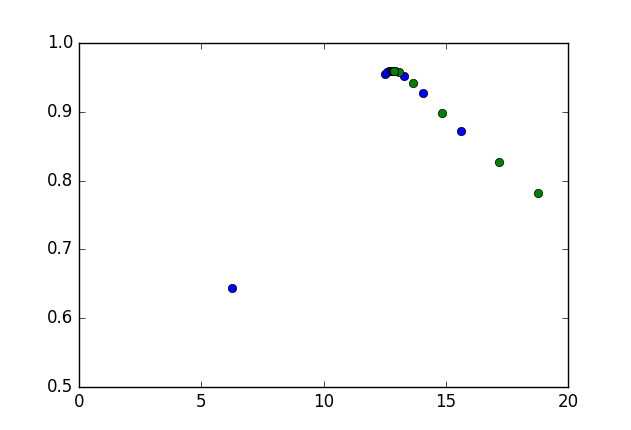
\includegraphics[scale=0.7]{python/ph2/iteration_COM/CT_x100_iteration_COM.png}
    \caption{CT x100, (4 steps lead to best result)}
    \label{fig:CT_x100_iteration}
  \end{subfigure}
  \begin{subfigure}[b]{1\textwidth}
    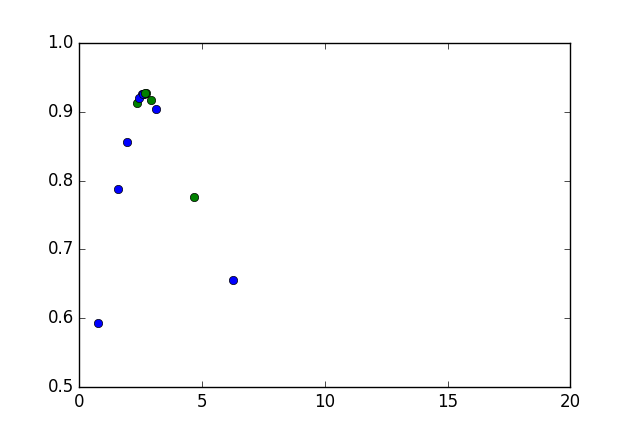
\includegraphics[scale=0.7]{python/ph2/iteration_COM/MR_x100_iteration_COM.png}
     \caption{MR x100, (15 steps performed)}
     \label{fig:MR_x100_iteration}
  \end{subfigure}
  \caption{COM iteration method}
  \label{fig:COM_iteration}
\end{figure}

% image of COM shift